\cotefile{133}
\scanpage{2}
\unsure{groupes} Witt

et formes \unsure{quadratiques}

\mspage{\unsure{1}}
\scanpage{3}
\[
q'\to q''\unsure{=}\unsure{q'''|q''''}= -1
\qquad q'''=q'\unsure{\circ}q''\unsure{\circ 1}
\]

\begin{center}
UNIVERSITE DES SCIENCES ET TECHNIQUES\\
DU LANGUEDOC\\
\rule{0.8cm}{0.4pt}\\
INSTITUT DE MATHEMATIQUES\\
Place Eugène Bataillon\\
34060 MONTPELLIER CEDEX\\
\rule{0.8cm}{0.4pt}
\end{center}

Montpellier, le

\[
\deleted{\unsure{C\times C\to C}}
\qquad \deleted{\unsure{C\times C\times}}
\qquad (\unsure{x}\otimes y)\otimes z\simeq x\otimes y\otimes z)
\]

\[
\deleted{L_\bullet\otimes\unsure{L'_\bullet}\otimes\unsure{L''}}
\]

\diagram{\begin{tikzcd}[ampersand replacement=\&,column sep=large,row sep=large]
(L_\bullet\otimes L_\bullet)\otimes L_\bullet
  \arrow[rr,"a"] \arrow[d,"{\unsure{p\otimes L_\bullet}}"'] \&\&
L_\bullet\otimes(L_\bullet\otimes L_\bullet) \arrow[d,"{L_\bullet\otimes p}"]\\
L_\bullet\otimes L_\bullet \arrow[dr,"p"'] \&
\deleted{\unsure{\alpha}} \& L_\bullet\otimes L_\bullet \arrow[dl,"p"]\\
\&L\&
\end{tikzcd}}

\diagram{\begin{tikzcd}[ampersand replacement=\&,column sep=large]
\operatorname{Ext}^1(\pi_0,\pi_0,\pi_0;\pi_1)\deleted{(L_\bullet\otimes L_\bullet)} \&
\operatorname{Ext}(\pi_0,\pi_0;\pi_1)\arrow[l,"{\delta^{(\unsure{1|2})}}"']
\end{tikzcd}}

\diagram{\begin{tikzcd}[ampersand replacement=\&,column sep=huge,row sep=large]
\unsure{((x\otimes y)\otimes z)\otimes t}\arrow[r]\arrow[d]\&
(x\otimes y)\otimes(z\otimes t)\arrow[dd,leftrightarrow,very thick]\\
(x\otimes(y\otimes z))\otimes t\arrow[d]\&\\
x\otimes((y\otimes z)\otimes t)\arrow[r]\&x\otimes(y\otimes(z\otimes t))
\end{tikzcd}}

\mspage{2}
\scanpage{4}
\[
P'=W^*(L^{\otimes 2})\qquad E=L+L^{-1}
\]
\[
\underbrace{L_{P'}^{\otimes2}\simeq\uline{O}_{P'}}_{\eta\in H^1(P',\mathbb F_2)}
\qquad Q(\unsure{x,x'})=\deleted{\unsure{xx'}}\ xx'
\]
\[
\eta^2+w_1\eta+w_2=0
\]

Je dis que
\[
\begin{aligned}
w_1&=\alpha\overset{\mathrm{df}}{=}\partial(-1)\\
w_2&\unsure{\equiv|=}c_1\bmod 2
\end{aligned}
\]
\margin{$\partial:H^0(S,G_m)\to H^1(S,\mu_2)$}

\[
\prod_i(1+\alpha+\unsure{\xi_i|\zeta_i})
\qquad
\begin{gathered}
(1+y)(1+y+\alpha)\\
1+\alpha+\underbrace{y(y+\alpha)}_{\substack{\unsure{\Vert|=}\\c_1\ ?}}
\end{gathered}
\]

\margin{$A\to B$\quad $M\quad N$}
\[
E_2^{pq}=\uline{\operatorname{Ext}}_{\unsure{B}}^p
(\operatorname{Tor}_{\unsure{q}}^A(M,B),N)
\]

\figure{\begin{tikzpicture}[x=1cm,y=1cm]
\draw (-0.7,0.04)--(0,0)--(0.85,0.02);
\draw (0,-0.65)--(0.04,0.55)--(0.06,1.4)--(0,1.65);
\draw (0.00,0.62)--(0.07,0.62);
\draw (0.02,1.25)--(0.11,1.25);
\draw (0.48,-0.04)--(0.48,0.05);
\fill (0.54,0.63) circle (0.025);
\fill (0.60,1.28) circle (0.025);
\end{tikzpicture}}

\diagram{$\begin{array}{rl}
\substack{\text{mercr.}\\22}&\left\{\begin{array}{lr}
\text{épicerie}&15,20\\
\text{pain}&12,30\\
\substack{\text{\unsure{beurre, bananes}}\\\text{œufs}}&9,40
\end{array}\right.\\[1em]
\text{\unsure{J. et D.}}&\left\{\begin{array}{lr}\text{bus}&22,\text{—}\\&\end{array}\right.
\end{array}$}

\mspage{3}
\scanpage{6}
Groupes de Witt et variantes.

$S$ topos loc. annelé

$WG(S)=$ groupe enveloppant du monoïde commutatif
 des classes d'isomorphie des modules quadratiques
 sur $S$ [loc. libres de r.f.] \uline{strictement} non
 dégénérés (i.e. la forme bil. ass. est non
 dégénérée)

\uline{NB} $WG(S)$ est un pré-$\lambda$-anneau
\inserted{(sans unité en général...)} augmenté vers
``l'anneau binomial'' $H^0(S,\mathbb Z)$ ($\simeq\mathbb Z$ si $S$ connexe)

Si $S$ connexe \deleted{\illegible{1}} (et $2$ non inversible dans $\uline{O}_S$,
alors $WG(S)\xrightarrow{\varepsilon}\mathbb Z$ prend ses valeurs dans $2\mathbb Z$
(les modules quadratiques str. non. dég. sont de
rang pair. Si $2$ est inversible \inserted{dans $\uline{O}_S$}, alors
$WG(S)$ est un anneau avec unité. Même
dans ce cas j'ignore si c'est un $\lambda$-anneau
(et pas seulement un pré-$\lambda$-anneau), donc
si on a les formules universelles
\[
\lambda^i(xy)=P_i(x,\deleted{\unsure{\lambda^2x}},-\,-\,\lambda^{\unsure{i-1|i}}x;
 y,\deleted{\unsure{\lambda^2y}},-\,-,\lambda^{\unsure{i-1|i}}y)\quad(i\ge2
\]
\[
\lambda^i(\lambda^j x)=Q_{i,j}(x,\lambda^2x,-\,-,\lambda^{ij}(x))
\qquad(i,j\ge2)
\]
($P_i$, $Q_{ij}$ pol. univ. à coeff. dans $\mathbb Z$...)

\uline{NB} Pour la première formule p.ex, il suffit de se
placer sur le topos classifiant d'un
groupe $O(m)\times O(n)$, en prenant pour $x$ et $y$
les classes des images inverses sur $B_{O(m)\times O(n)}$
des \deleted{\unsure{fib}} modules quadratiques universels
\deleted{de} rang $m$ resp. $n$ sur $B_{O(m)}$ resp $B_{O(n)}$.
Cela nous amène donc à étudier $WG(B_{O(m)\times O(n)})$
\unsure{De =} la deuxième formule à \deleted{\unsure{donc}}\deleted{\unsure{vérifier}} dans
un $B_{O(m)}$, d'où la tâche de déterminer
\[
WG(B_{O(m)})
\]

\mspage{5}
\scanpage{7}
On a un hom. de groupes
\[
K_s(S)\xrightarrow{\alpha}WG(S)
\]
en associant à la classe du \deleted{fibré} Module loc. libre $E$ \inserted{de r.f.}
le \deleted{\unsure{fib}} module quadratique $E\oplus\check E$, avec la forme
$\unsure{q(a,a')=\langle a,a'\rangle}$ ; ici $K_s(S)$ désigne le groupe $K$
``spécial'', groupe enveloppant du monoïde des
classes d'isomorphie de modules loc. lib. de r.f. sur $S$;
il n'est pas clair que l'hom. précédent se factorise
par $K(S)$ (déduit de $K_s(S)$ en tenant compte des
suites exactes courtes...)

(\unsure{donc} si $E$ est ext. \inserted{non splittée} de $E'$ par $E''$, il n'est pas clair
si on a $\varphi(E)=\varphi(E')+\varphi(E'')$ dans $WG(S)$....)

Par définition, $W(S)$ (groupe de Witt) est le conoyau
de l'hom. précédent
\[
K_s(S)\xrightarrow{\alpha}WG(S)\longrightarrow W(S)\longrightarrow0
\]

\uline{NB} Si $2$ inv. dans $\uline{O}_S$, alors pour tt \unsure{Module} quadratique
$(M,q)$, la somme $F=(M,q)\oplus(M,-q)$ définit \unsure{cet} \unsure{élément}
nul de $W(S)$, i.e. est $\simeq$ à un $E\oplus\check E$ comme
dessus : il suffit de prendre $E=M$, immergé
dans $F$ diagonalement et anti diagonalement
[en fait, les \inserted{mod. quad.} $F$ de la forme $(M,q)\oplus(M,-q)$ sont,
à isom. près, \deleted{\unsure{les}} de la forme $E\oplus\check E$...,
mais où $E$ est un Mod. loc. lib. de r.f.
qui admet (au moins une) forme quadratique
(str.) non dégénérée.

\unsure{De =}, si $S$ est un schém. affine, il

\mspage{6}
\scanpage{8}
paraît (\unsure{Laborde|Lazard} dixit) que (sans condition que
$2$ soit inversible) les modules $(M,q)\oplus(M,-q)$
sont de la forme \inserted{$\alpha(E)=$} $E\oplus\check E$. (Mais ce n'est pas
\deleted{Dans}
vrai dans \deleted{\unsure{tout}} \inserted{le} cas d'un topos loc. annelé —
p.ex. cela n'est pas vrai pour le topos classifiant
$B_{O(n)}$ si $n\ge1$)

\margin{à vérifier}
Dans l'un et l'autre cas, $W(S)$ peut
dès lors se construire directement comme
quotient de l'ens des classes d'isom.
de modules quadratiques, avec
$(M,q)\sim(M',q')$ si \deleted{$(M,q)\oplus(M',-q')$}
\deleted{est isom. à un $E\oplus\check E$} \inserted{$=\alpha(E)$}
$\exists$ Mod loc. lib. de r.f. $E,F$ avec
\[
(M,q)\oplus(M',-q')+\alpha(F)\simeq\alpha(E)
\]

[\uline{NB} Si $F$ est \unsure{isom.} à un fact direct de $E$,
\inserted{et si on dispose d'un ``th de Witt''}
— ce qui est tjrs le cas si $S$ est le spectre d'
un corps — \deleted{et si} alors cette condition signifie
aussi que $\exists G$ loc. lib de r.f. tel que
\[
(M,q)\oplus(M',-q')\simeq\alpha(G)
\]
]

On voit que $\alpha(K(S))$ est un \uline{idéal} dans
$WG(S)$ : donc $W(S)$ est encore un anneau.
Mais il n'est plus augmenté vers $H^0(S,\mathbb Z)$,
seulement vers $H^0(S,\underbrace{\mathbb Z/2\mathbb Z}_{\mathbb F_2})$ (donc vers
$\mathbb F_2$ si $S$ connexe $\ne\varnothing$). Mais que peut-on
dire de la pré-$\lambda$-structure de $WG(S)$
— passerait-elle au quotient ?

\mspage{7}
\scanpage{9}
On suppose maintenant pour simplifier que
l'Anneau $\uline{O}_S$ est \unsure{\uline{strict\textsuperscript{mt}}} \uline{local}
\inserted{(p.ex. anneau \unsure{faisceau dans} top. ét)}. On dispose alors
\margin{\unsure{On supp.} de plus $2$ inv. dans $\uline{O}_S$}
\[
WG(S)\xrightarrow{w}H^*(S,\mathbb F_2)
\]
(classes de Stiefel Whitney), caractérisé (pour
$S$ variable) par

a) \uline{fonctorialité} en $S$

b) $\unsure{w(M,q)}$ dans le cas où $M$ de rang $1$
(normalisation)

c) $w(x+y)=w(x)w(y)$
\[
w(\unsure{x|m})-1\in H^+(S,\mathbb F_2)\qquad\text{i.e. }w^0(x)=1.
\]

\margin{\deleted{\unsure{par splitting} \unsure{on se ramène à} \unsure{prouver}
$w(\alpha(E))=1$, $E$ de rang $1$.}}
\deleted{Un calcul facile montre que $w\circ\alpha=1$, donc
$w$ se factorise en}
\deleted{\[
W(S)\xrightarrow{w}1+\widehat H^{*+}(S,\mathbb F_2)
\]}

\deleted{\uline{NB} $w(M,q)$ \illegible{3} \unsure{que}}

\uline{NB} Les arguments habituels de splitting
montrent que $w(M\otimes N)$ et $w(\lambda^{\unsure{i}}M)$ se
calculent par les formules \inserted{universelles} habituelles en
termes de $w(M),w(N)$ et $\rho(M),\rho(N)$ (rangs
des Modules $M,N$). Donc on a un \inserted{$\lambda$-}hom
\[
WG(S)\longrightarrow H^0(S,\mathbb Z)\times\deleted{\unsure{H}}(1+\widehat H^{*+}(S,\mathbb F_2))
\]

\mspage{8}
\scanpage{11}
\textbf{C. R. Acad. Sc. Paris, t. 279 (16 septembre 1974)}\hfill\textbf{Série A — 447}

\rule{\linewidth}{0.4pt}

ALGÈBRE. — \emph{Théorème de Skolem-Nother pour les algèbres d'Azumaya
graduées sur un anneau semi-local.} Note (*) de M. \textbf{Olivier Laborde},
présentée par M. René Garnier.

Le théorème de Skolem-Nother se généralise au cas des algèbres d'Azumaya graduées grâce
à quelques propriétés des anneaux gradués simples et semi-simples. Une première application
à la K-théorie de ce résultat est la régularité de ces algèbres pour le produit tensoriel.

1. \textsc{Modules et anneaux gradués semi-simples}. — Un anneau, A, est gradué si additivement,
il est une somme directe de sous-groupes $\mathrm A=\mathrm A_0\oplus\mathrm A_1$ qui, pour la multiplication
vérifient les inclusions $\mathrm A_i.\mathrm A_j\subseteq\mathrm A_{i+j}$ ($i,j\in\mathbf Z/2\mathbf Z$). On notera $|\mathrm A|$ l'anneau sous-jacent
non gradué.

Un A-module gradué, M, est un $|\mathrm A|$-module qui est pour l'addition une somme directe
$\mathrm M=\mathrm M_0\oplus\mathrm M_1$ qui satisfait $\mathrm A_i\,\mathrm M_j\subseteq\mathrm M_{i+j}$ ($i,j\in\mathbf Z/2\mathbf Z$) et $|\mathrm M|$ sera le $|\mathrm A|$-module
sous-jacent non gradué.

Dans ce qui suit les anneaux, les idéaux, les algèbres et les modules seront, sauf mention
expresse du contraire, gradués et on les appellera des Anneaux, des Idéaux, des Algèbres
et des Modules. Pour d'autres renseignements, \emph{voir} (${}^3$).

\textsc{Définition 1}. — Un A-Module à gauche M est Simple si les seuls sous-Modules de M
sont $\{0\}$ et M.

\textsc{Proposition 1}. — \emph{Un A-module à gauche Simple non nul est de la forme
$\mathrm A\,\unsure{s/}\mathbf m$ où $\mathbf m$
est un Idéal à gauche maximal de} A.

\emph{Preuve}. — Il est immédiat que $\mathrm A\,\unsure{s/}\mathbf m$ est Simple. Réciproquement, soit M un A-Module
Simple et $x$ un élément homogène non nul de M. Considérons l'application $f$ qui à $\alpha\in\mathrm A$
fait correspondre $\alpha x\in\mathrm M$. Le noyau de $f$ est un Idéal de A quel que soit le degré de $x$ :
Si $\alpha\in\operatorname{Ker}(f)$, on a
\[
\alpha x=\alpha_0x+\alpha_1x=0\quad\Rightarrow\quad\alpha_0x=\alpha_1x=0
\qquad\text{et}\qquad\alpha_0\text{ et }\alpha_1
\]
appartiennent eux aussi à $\operatorname{Ker}(f)$.

\textsc{Lemme}. — \emph{Soit} M \emph{un A-Module qui est somme d'une famille}
$(\mathrm M_i)_{i\in\unsure{i|I}}$ \emph{de sous-Modules
Simples et} F \emph{un sous-Module de} M. \emph{Alors il existe}
$\mathrm J\subseteq\mathrm I$ \emph{tel que}
$\mathrm M=\mathrm F\oplus\bigoplus_{j\in\mathrm J}\mathrm N_j$.

La démonstration est identique à celle du cas non gradué.

\textsc{Proposition 2}. — \emph{Soit} M \emph{un A-Module. Les propositions suivantes sont équivalentes} :

\emph{(a)} M \emph{est somme d'une famille de sous-Modules Simples.}

\emph{(b)} M \emph{est somme directe d'une famille de sous-Modules Simples.}

\emph{(c) Tout sous-Module de} M \emph{est facteur direct.}

\emph{Preuve}. — Elle est rendue immédiate par le lemme précédent.

\textsc{Définition 2}. — On dira qu'un A-module M est Semi-Simple s'il vérifie l'une des conditions
équivalentes de la proposition 2.

\mspage{10}
\scanpage{12}
\textbf{448 — Série A}\hfill\textbf{C. R. Acad. Sc. Paris, t. 279 (16 septembre 1974)}

\rule{\linewidth}{0.4pt}

\textsc{Proposition 3}. — \emph{Tout sous-Module et tout Module quotient d'un Module Semi-Simple
est encore Semi-Simple.}

\emph{Preuve}. — Elle est analogue à celle rencontrée dans le cas des modules semi-simples
non gradués.

\textsc{Définition 3}. — On appelle Radical de A et on note $\operatorname{Rad}(\mathrm A)$ l'intersection des Idéaux
à gauche maximaux de A. Le fait que $\operatorname{Rad}(\mathrm A)$ soit égal à l'intersection des annulateurs
des A-Modules Simples montre que c'est un Idéal bilatère. (Un élément $\alpha$ de A appartient
à l'annulateur de tout A-Module Simple $\Leftrightarrow$ $\alpha$ est l'annulateur de tout élément homogène
d'un A-Module Simple $\Leftrightarrow$ $\alpha$ appartient à tous les Idéaux à gauche maximaux de A.)

\textsc{Proposition 4}. — \emph{Soit $k$ un corps commutatif. Une $k$-algèbre Simple de dimension finie
est Semi-Simple.}

\emph{Preuve}. — Soit $\mathbf r$ un élément minimal de l'ensemble des intersections finies d'Idéaux à
gauche minimaux de A. Si $\mathbf m$ est un Idéal à gauche maximal de A, on a $\mathbf m\cap\mathbf r=\mathbf r$ d'où
$\mathbf r\subseteq\mathbf m\Rightarrow\mathbf r\subseteq\operatorname{Rad}(\mathrm A)$ ce qui entraîne que $\mathbf r=0$ vu que $\operatorname{Rad}(\mathrm A)$ est un idéal bilatère. Il
existe donc une famille finie $(\mathbf m_i)_{1\le i\le n}$ d'Idéaux à gauche maximaux dont l'intersection
est nulle. L'anneau A s'injecte dans le produit des $\mathrm A/\mathbf m_i$ et $\unsure{\mathrm A\,s|\mathrm A_s}$ est par conséquent semi-simple.

\textsc{Proposition 5}. — \emph{Une $k$-Algèbre Simple} A \emph{de dimension finie sur un corps $k$ est telle
que tout A-Module soit isotypique de type} A.

\emph{Preuve}. — D'après la proposition précédente, nous savons déjà que A est semi-simple.
Les Idéaux bilatères de A sont des sous-modules de $\unsure{\mathrm A\,s|\mathrm A_s}$ stables par multiplication à droite,
donc stables par le commutant de $\unsure{\mathrm A\,s|\mathrm A_s}$ qui n'est autre que l'anneau des homothéties à
droite de A ($\mathrm C\in\mathcal L_{\mathrm A}(\unsure{\mathrm A\,s|\mathrm A_s})$, $\mathrm C(y)=\mathrm C(\unsure{y_1|y1})=y\,\mathrm C(1)$). Ce sont donc des sommes de composants
isotypiques de $\unsure{\mathrm A\,s|\mathrm A_s}$ [(${}^1$), p. 34]. En particulier, les composants isotypiques de $\unsure{\mathrm A\,s|\mathrm A_s}$
sont les Idéaux bilatères minimals de A et la proposition en résulte.

2. \textsc{Théorème de Skolem-Nother}.

\textsc{Théorème 1}. — \emph{Soit $k$ un corps commutatif,} A \emph{une $k$-Algèbre Centrale Simple,} B \emph{une
$k$-Algèbre Simple, $f$ et $g$ deux homomorphismes de} B \emph{dans} A. \emph{Alors il existe un élément
$s\in\mathrm U(\mathrm A_0)$ (groupe des éléments inversibles de $\mathrm A_0$) qui est tel que pour tout $b\in\mathrm B$, on ait}
\[
f(b)=s^{-1}g(b)s.
\]

\emph{Preuve}. — On suppose d'abord que $\mathrm A=\operatorname{END}(\mathrm V)$ où V est un A-Module. On munit V
de deux structures de B-Module :
\[
b.v=f(b)(v)\qquad\text{et}\qquad b.v=g(b)(v).
\]

On voit que $\mathrm B_i\,\mathrm V_i\subseteq\mathrm V_{i+j}$ et que $\mathrm V_f$ et $\mathrm V_g$ ont même dimension sur $k$ et la proposition 5
nous montre que $\mathrm V_f$ et $\mathrm V_g$ sont des B-Modules isomorphes. On a
\[
s\in\mathrm U(\mathrm A_0)\qquad\text{avec}\qquad s(f(b)(v))=g(b)s(v)
\]
quels que soient $b\in\mathrm B$ et $v\in\mathrm V$ d'où
\[
f(b)(v)=s^{-1}\circ g(b)\circ s(v).
\]

\mspage{11}
\scanpage{13}
\textbf{C. R. Acad. Sc. Paris, t. 279 (16 septembre 1974)}\hfill\textbf{Série A — 449}

\rule{\linewidth}{0.4pt}

Pour traiter le cas général, rappelons que vu l'hypothèse faite sur A, les Algèbres $\mathrm A\otimes\mathrm A^*$
et $\operatorname{END}(\mathrm A)$ sont isomorphes. Par composition nous obtenons deux isomorphismes

\diagram{\begin{tikzcd}[ampersand replacement=\&]
\mathrm B\otimes\mathrm A\arrow[r,shift left=0.5ex,"{f\otimes1}"]\arrow[r,shift right=0.5ex,"{g\otimes1}"']\&
\mathrm A\otimes\mathrm A^*\arrow[r,"\tau"]\&\operatorname{END}(\mathrm A).
\end{tikzcd}}

Il existe donc $\bar s\in\mathrm U[(\mathrm A\otimes\mathrm A^*)_0]$ tel que
\[
\bar s^{-1}(g(b)\otimes a^*)\bar s=f(b)\otimes a^*.
\]
En donnant à $b$ la valeur 1, on voit que
\[
1\otimes a^*.\bar s=\bar s.1\otimes a^*.
\]
Mais nous savons que
\[
\mathrm C_{\mathrm A^*}(1\otimes\mathrm A^*)=1\otimes\mathrm Z(\mathrm A^*)=\mathrm A\otimes k=\mathrm A\otimes1
\]
ce qui montre que $\bar s=s\otimes1$ où $s\in\mathrm A_0$. Nous voyons que $\bar s^{-1}=t\otimes1$ et par conséquent
$s\in\mathrm U(\mathrm A_0)$. En décomposant $\bar s$, en faisant $a=1$, on a le résultat souhaité compte tenu de
\[
\mathrm A\simeq\mathrm A\otimes1\subseteq\mathrm A\otimes\mathrm A^*=\mathrm A^e.
\]

\textsc{Théorème 2}. — \emph{Soit} R \emph{un anneau commutatif semi-local,} A \emph{et} B \emph{deux R-Algèbres d'Azumaya.
Si $f$ et $g$ sont deux homomorphismes d'Algèbres injectifs de} B \emph{dans} A, \emph{il existe un
automorphisme intérieur $\theta$ induit par un élément de degré} 0 \emph{de} A \emph{tel que $f=\theta\circ g$.}

\emph{Preuve}. — Comme dans (${}^2$), on commence par démontrer ce résultat pour un produit
fini de corps, puis on considère les homomorphismes induits $\bar f$, $\bar g$ de $\mathrm B/\operatorname{Rad}(\mathrm R)\,\mathrm B$ dans
$\mathrm A/\operatorname{Rad}(\mathrm R)\,\mathrm A$. L'automorphisme intérieur $\bar\theta$ de $\mathrm A/\operatorname{Rad}(\mathrm R)\,\mathrm A$ se remonte en un automorphisme
$\theta$ de A.

3. \textsc{Régularité des algèbres d'Azumaya graduées}.

\textsc{Théorème 3}. — \emph{Soit} R \emph{un anneau semi-local,} A, B \emph{et} C \emph{des R-algèbres d'Azumaya telles
qu'il existe un isomorphisme $h$ entre $\mathrm A\otimes\mathrm C$ et $\mathrm B\otimes\mathrm C$. Alors il existe un isomorphisme
entre} A \emph{et} B.

\emph{Preuve}. — Il suffit de considérer les deux homomorphismes

\diagram{\begin{tikzcd}[ampersand replacement=\&]
\mathrm C\arrow[r]\arrow[d]\&1\otimes\mathrm C\arrow[r]\&\mathrm A\otimes\mathrm C\arrow[d]\\
1\otimes\mathrm C\arrow[rr]\&\&\mathrm B\otimes\mathrm C
\end{tikzcd}}

et d'appliquer le théorème de Skolem-Nother.

(*) Séance du 24 juin 1974.

(${}^1$) N. \textsc{Bourbaki}, \emph{Modules et anneaux semi-simples}, Hermann, Paris, 1958.

(${}^2$) A. \textsc{Roy} et R. \textsc{Sridharan}, \emph{J. Math. Kyoto Univ.}, \textbf{7-2}, 1967, p. 161-167.

(${}^3$) C. \textsc{Small}, \emph{Trans. Amer. Math. Soc.}, \textbf{156}, 1971, p. 455-491.

\begin{flushright}
\emph{Université des Sciences}\\
\emph{et des Techniques du Languedoc,}\\
\emph{U. E. R. de Mathématiques,}\\
\emph{place Eugène-Bataillon,}\\
34060 \emph{Montpellier.}
\end{flushright}

\mspage{12}
\scanpage{14}
\textbf{C. R. Acad. Sc. Paris, t. 278 (24 juin 1974)}\hfill\textbf{Série A — 1599}

\rule{\linewidth}{0.4pt}

ALGÈBRE. — \emph{Formes quadratiques, algèbres de Clifford et signatures.}

Note (*) de M. \textbf{Olivier Laborde}, présentée par M. René Garnier.

Détermination du noyau de l'homomorphisme du groupe de Witt d'un corps de nombres ou
d'un anneau d'entiers algébriques dans le groupe de Brauer-Wall. Le calcul du groupe de Witt
est ramené à celui de $\mathrm K^*/\mathrm K^{*2}$ pour un corps de nombres et à celui du groupe des extensions
quadratiques pour un anneau d'entiers algébriques.

1. \textsc{Introduction}. — Étant donné un anneau commutatif unitaire A, il existe un homomorphisme
de groupe $f_{\mathrm A}$ de $\operatorname{Witt}(\mathrm A)$ dans $\operatorname{BW}(\mathrm A)$ définit dans (${}^2$) comme suit : si $q$ est
une forme quadratique non dégénérée sur un A-module projectif de type fini P, on note $[q]$
sa classe d'équivalence dans $\operatorname{Witt}(\mathrm A)$ et si D est une A-algèbre d'Azumaya graduée,
on note $[\mathrm D]$ sa classe d'équivalence dans $\operatorname{BW}(\mathrm A)$; alors $f_{\mathrm A}([q])=[\mathrm C(q)]$. L'image
de cet homomorphisme s'appelle le groupe de Hasse-Wall de A et on le note $\operatorname{HW}(\mathrm A)$;
le caractère fonctoriel de Witt, BW, HW et $f$ sera utilisé. D'après (${}^6$), si A est un anneau
de Dedekind dont le corps de fractions est tel que toute forme quadratiques de plus de
cinq variables soit isotrope, les groupes $\operatorname{Witt}(\mathrm A)$ et $\operatorname{HW}(\mathrm A)$ sont isomorphes.

En outre, dans (${}^9$), il est démontré que si K est un corps tel que les groupes $\operatorname{Witt}(\mathrm K)$
et $\operatorname{HW}(\mathrm K)$ soient isomorphes, alors le corps K possède la propriété indiquée ci-dessus.

Dans ce qui suit, nous déterminerons le noyau $\operatorname{LW}(\mathrm A)$ de l'homomorphisme $f_{\mathrm A}$ lorsque A
est un corps de nombres algébriques ou l'anneau de ses entiers et nous indiquerons à quels
invariants se ramène le calcul du groupe de Hasse-Wall.

Ce travail a été inspiré par (${}^7$).

2. \textsc{Les corps de nombres}. — Soit K un corps de nombre, i. e. une extension algébrique
finie du corps Q des nombres rationnels. Nous partagerons l'ensemble $\Omega$ des valuations
de K de la façon suivante :

(i) \emph{Les valuations réelles} (en nombre fini) : Ces valuations $(r_i)_{1\le i\le r}$ définissent sur K
une structure d'espace topologique et les complétés $\mathrm K_{r_i}$ sont isomorphes au corps des
nombres réels.

(ii) \emph{Les valuations complexes et les valuations discrètes} (en nombre infini) : Ces
valuations $(c_j)_{j\in\mathrm J}$ définissant sur K une structure d'espace topologique dont les complétés $\mathrm K_{c_j}$
sont isomorphes dans le cas des valuations complexes au corps des nombres complexes
et dans le cas des valuations discrètes à un corps local de caractéristique nulle, c'est-à-dire
dans ce cas une extension finie d'un corps $p$-adique.

A chaque valuation $v$ de K correspond une application de K dans $\mathrm K_v$. Le caractère
fonctoriel des groupes Witt et HW nous conduit au diagramme

\diagram{\begin{tikzcd}[ampersand replacement=\&,column sep=small]
0\arrow[r]\&\operatorname{LW}(\mathrm K)\arrow[r]\arrow[d,"\alpha"']\&
\operatorname{Witt}(\mathrm K)\arrow[r]\arrow[d,"\beta"']\&
\operatorname{HW}(\mathrm K)\arrow[r]\arrow[d,"\gamma"']\&0\\
0\arrow[r]\&\displaystyle\prod_{v\in\Omega}\operatorname{LW}(\mathrm K_v)\arrow[r]\&
\displaystyle\prod_{v\in\Omega}\operatorname{Witt}(\mathrm K_v)\arrow[r]\&
\displaystyle\prod_{v\in\Omega}\operatorname{HW}(\mathrm K_v)\arrow[r]\&0
\end{tikzcd}}

\textbf{C. R., 1974, 1\textsuperscript{er} \emph{Semestre}. (T. 278, N\textsuperscript{o} 26)}\hfill\textbf{Série A — 115}

\mspage{13}
\scanpage{15}
\textbf{1600 — Série A}\hfill\textbf{C. R. Acad. Sc. Paris, t. 278 (24 juin 1974)}

\rule{\linewidth}{0.4pt}

\textsc{Proposition 1}. — \emph{L'application $\alpha$ est un isomorphisme et nous avons la suite exacte} :

\diagram{\begin{tikzcd}[ampersand replacement=\&]
0\arrow[r]\&(8\mathbf Z)^r\arrow[r]\&\operatorname{Witt}(\mathrm K)\arrow[r]\&\operatorname{HW}(\mathrm K)\arrow[r]\&0
\end{tikzcd}}

\emph{où $r$ est le nombre de valuations réelles de} K.

\emph{Preuve}. — L'application $\beta$ est injective d'après le théorème de Hasse-Minkowski et
il en est de même de l'application $\alpha$. D'autre part, si $v$ est une valuation du type (i),
$\operatorname{LW}(\mathrm K_v)\cong8\mathbf Z$, et si elle est du type (ii), $\operatorname{LW}(\mathrm K_v)=\{0\}$. Par conséquent,
$\displaystyle\prod_{v\in\Omega}\operatorname{LW}(\mathrm K)\cong(8\mathbf Z)^r$. Le fait que $\alpha$ soit surjective résulte de la théorie classique des formes
quadratiques sur un corps de nombres [\emph{cf.} (${}^3$), p. 413 par exemple]\quad$\blacksquare$

D'après (${}^6$) ou (${}^7$), nous avons la suite exacte :

\diagram{\begin{tikzcd}[ampersand replacement=\&]
0\arrow[r]\&\mathrm N(\mathrm K)\arrow[r]\&\operatorname{HW}_0(\mathrm K)\arrow[r]\&\mathrm K^*/\mathrm K^{*2}\arrow[r]\&0
\end{tikzcd}}

où $\mathrm N(\mathrm K)$ est un sous-groupe de $\operatorname{Br}(\mathrm K)$ constitué d'éléments d'exponent deux de $\operatorname{Br}(\mathrm K)$
et $\operatorname{HW}_0(\mathrm K)$ l'image par $f_{\mathrm K}$ du sous-groupe $\operatorname{Witt}_0(\mathrm K)$ obtenu à partir des formes quadratiques
de rang pair.

On vérifie sans peine à l'aide de la s. e. [\emph{cf.} (${}^{10}$)] :

\diagram{\begin{tikzcd}[ampersand replacement=\&]
0\arrow[r]\&\operatorname{Br}(\mathrm K)\arrow[r]\&
\displaystyle\unsure{\bigoplus|\bigotimes}_{v\in\Omega}\operatorname{Br}(\mathrm K_v)\arrow[r]\&\mathbf Q/\mathbf Z\arrow[r]\&0
\end{tikzcd}}

et du résultat rappelé dans la démonstration de la proposition 1 que $\mathrm N(\mathrm K)=\operatorname{Br}^2(\mathrm K)$.
Le calcul de $\operatorname{Witt}(\mathrm K)$ est bien ramené à celui de $\mathrm K^*/\mathrm K^{*2}$.

3. \textsc{Les anneaux d'entiers algébriques}. — Soient K un corps de nombres et A l'anneau
des éléments de K entiers sur Z dont le corps de fractions est K.

Nous allons étudier le diagramme

\diagram{\begin{tikzcd}[ampersand replacement=\&,column sep=small]
0\arrow[r]\&\operatorname{LW}(\mathrm A)\arrow[r]\arrow[d,"a"']\&\operatorname{Witt}(\mathrm A)\arrow[r]\arrow[d,"b"']\&\operatorname{HW}(\mathrm A)\arrow[r]\arrow[d,"c"']\&0\\
0\arrow[r]\&\operatorname{LW}(\mathrm K)\arrow[r]\&\operatorname{Witt}(\mathrm K)\arrow[r]\&\operatorname{HW}(\mathrm K)\arrow[r]\&0
\end{tikzcd}}

\textsc{Lemme 1}. — \emph{L'application $c$ de $\operatorname{HW}(\mathrm A)$ dans $\operatorname{HW}(\mathrm K)$ est injective.}

\emph{Preuve}. — Considérons les diagrammes

\diagram{\begin{tikzcd}[ampersand replacement=\&,column sep=small]
0\arrow[r]\&\mathrm N(\mathrm A)\arrow[r]\arrow[d]\&\operatorname{HW}_0(\mathrm A)\arrow[r]\arrow[d]\&\mathrm Q(\mathrm A)\arrow[r]\arrow[d]\&0\\
0\arrow[r]\&\mathrm N(\mathrm K)\arrow[r]\&\operatorname{HW}_0(\mathrm K)\arrow[r]\&\mathrm Q(\mathrm K)\arrow[r]\&0
\end{tikzcd}}

et

\diagram{\begin{tikzcd}[ampersand replacement=\&]
0\arrow[r]\&\mathrm N(\mathrm A)\arrow[r]\arrow[d]\&\operatorname{Br}(\mathrm A)\arrow[d]\\
0\arrow[r]\&\mathrm N(\mathrm K)\arrow[r]\&\operatorname{Br}(\mathrm K)
\end{tikzcd}}

Il est montré dans (${}^1$) que $\operatorname{Br}(\mathrm A)$ est un sous-groupe de $\operatorname{Br}(\mathrm K)$ car A est un anneau de
Dedekind. D'autre part, le groupe $\mathrm Q(\mathrm R)$ d'un anneau quelconque R est identique au groupe

\mspage{14}
\scanpage{16}
\textbf{C. R. Acad. Sc. Paris, t. 278 (24 juin 1974)}\hfill\textbf{Série A — 1601}

\rule{\linewidth}{0.4pt}

$\mathrm T(\mathbf Z/2\mathbf Z,\mathrm R)$ définit dans (${}^5$) comme on le voit grâce au corollaire (7.4) de (${}^{11}$). D'après
le théorème 1 de (${}^5$), $\mathrm Q(\mathrm A)$ est un sous-groupe de $\mathrm Q(\mathrm K)$ car A est intégralement clos.
On conclut à l'aide du petit lemme des cinq\quad$\blacksquare$

\textsc{Lemme 2}. — \emph{L'application $a$ de $\operatorname{LW}(\mathrm A)$ dans $\operatorname{LW}(\mathrm K)$ est surjective.}

\emph{Preuve}. — D'après (${}^3$), théorème 5 et remarque, une forme quadratique Q sur K provient
d'une forme quadratique $q$ sur A si et seulement si les trois conditions suivantes sont
vérifiées :

(i) La dimension de Q est paire.

(ii) Son discriminant, i. e. le commutant de $\mathrm C_0(\mathrm Q)$ dans $\mathrm C(\mathrm Q)$ est de la forme $\mathrm S\underset{\mathrm A}{\otimes}\mathrm K$
où $\mathrm S\in\mathrm Q(\mathrm A)$.

(iii) Son algèbre de Clifford $\mathrm C(\mathrm Q)$ est de la forme $\mathrm D\underset{\mathrm A}{\otimes}\mathrm K$ où D est une A-algèbre
centrale séparable.

La condition (i) est vérifiée car la proposition 1 nous dit que si $\mathrm Q\in\operatorname{LW}(\mathrm K)$ elle est
le rang pair car ce groupe est isomorphe à $(8\mathbf Z)^r$.

Les conditions (ii) et (iii) sont immédiatement vérifiées car $[\mathrm C(\mathrm Q)]=[0]$.

Il existe donc une forme $q$ sur A telle que $b([q])=[\mathrm Q]$.

L'application $c$ étant injective, $[\mathrm C(q)]=[0]$ et donc $[q]\in\operatorname{LW}(\mathrm A)$\quad$\blacksquare$

\textsc{Proposition 2}. — \emph{L'application $a$ de $\operatorname{LW}(\mathrm A)$ dans $\operatorname{LW}(\mathrm K)$ est un isomorphisme et on
obtient la s. e. $0\to(8\mathbf Z)^r\to\operatorname{Witt}(\mathrm A)\to\operatorname{HW}(\mathrm A)\to0$ où $r$ est le nombre de valuations
réelles de} K.

\emph{Preuve}. — La proposition 2 de (${}^6$) montre que $b$ est injective. Il en est de même de $a$
et la proposition résulte des lemmes 1 et 2\quad$\blacksquare$

Nous avons la s. e. $0\to\mathrm N(\mathrm A)\to\operatorname{HW}(\mathrm A)\to\mathrm Q(\mathrm A)\to0$, où $\mathrm N(\mathrm A)$ est un sous-groupe
de $\operatorname{Br}^2(\mathrm A)$. A. Grothendieck a montré dans (${}^4$) que $\operatorname{Br}(\mathrm A)=(\mathbf Z/2\mathbf Z)^n$ où
$n=\operatorname{Max}\{0,r-1\}$. Soit $[\mathrm D]$ un élément de $\operatorname{Br}(\mathrm A)$. D'après le résultat rappelé au
paragraphe 2, l'algèbre $\mathrm D\underset{\mathrm A}{\otimes}\mathrm K$ est isomorphe à l'algèbre de Clifford $\mathrm C(\mathrm Q)$ d'une forme
de rang pair sur K. Les conditions (i), (ii), (iii) du théorème 5 de (${}^3$) sont donc vérifiées
et il existe une forme quadratique $q$ sur A telle que $\mathrm Q\cong q\underset{\mathrm A}{\otimes}\mathrm K$. Nous avons donc
\[
\mathrm D\underset{\mathrm A}{\otimes}\mathrm K\cong\mathrm C(\mathrm Q)\cong\mathrm C(q\underset{\mathrm A}{\otimes}\mathrm K)\cong\mathrm C(q)\underset{\mathrm A}{\otimes}\mathrm K.
\]

Comme $\operatorname{Br}(\mathrm A)$ s'injecte dans $\operatorname{Br}(\mathrm K)$, on a $[\mathrm D]=[\mathrm C(q)]$. Il en résulte que $\mathrm N(\mathrm A)=\operatorname{Br}(\mathrm A)$.
La suite exacte $0\to(\mathbf Z/2\mathbf Z)^n\to\operatorname{HW}(\mathrm A)\to\mathrm Q(\mathrm A)\to0$ ramène donc le calcul de $\operatorname{Witt}(\mathrm A)$
à celui de $\mathrm Q(\mathrm A)$.

\emph{Exemples} :

1\textsuperscript{o} $\mathrm A=\mathbf Z$ :
\[
\operatorname{Br}(\mathbf Z)=\mathrm Q(\mathbf Z)=0\qquad\text{et}\qquad r=1.
\]

D'où $\operatorname{HW}(\mathbf Z)=0$ et $\operatorname{Witt}(\mathbf Z)=8\mathbf Z$ [\emph{cf.} (${}^7$) et (${}^8$)].

\mspage{15}
\scanpage{17}
1602 --- Série A \hfill C. R. Acad. Sc. Paris, t. 278 (24 juin 1974)

\figure{\begin{tikzpicture}\draw (0,0)--(12,0);\end{tikzpicture}}

$2^\circ\ \mathrm{A}=\mathbf{Z}[i]$ :
\[
\operatorname{Br}(\mathbf{Z}[i])=\mathrm{Q}(\mathbf{Z}[i])=0\qquad\text{et}\qquad r=0.
\]
D'où $\mathrm{HW}(\mathbf{Z}[i])=\operatorname{Witt}(\mathbf{Z}[i])=0$.

(*) Séance du 4 février 1974.

(${}^1$) M. \textsc{Auslander} et O. \textsc{Goldmann}, \textit{Trans. Amer. Math. Soc.}, 97, 1960, p. 376-409.

(${}^2$) H. \textsc{Bass}, \textit{Topics in algebraic K-theory}, Tata Institute of Fundamental Research. Bombay, 1966.

(${}^3$) A. \textsc{Fröhlich}, \textit{Quart. J. Math.}, Oxford, (2), 22, 1971, p. 401-423.

(${}^4$) A. \textsc{Grothendieck}, \textit{Le groupe de Brauer III. Dix exposés sur la cohomologie des schémas}, North-Holland, 1968.

(${}^5$) D. \textsc{Harrison}, \textit{Abelian Extensions of Commutative Rings}, A. M. S. Memoirs, 1965, p. 68-79.

(${}^6$) O. \textsc{Laborde}, \textit{Bull. Sc. math.}, $2^{\mathrm e}$ série, 96, 1972, p. 199 à 208.

(${}^7$) A. \textsc{Larotonda}, A. \textsc{Micali} et O. E. \textsc{Villamayor}, \textit{Sur le groupe de Witt}, Istituto Nazionale di Alta Matematica (\textit{Symposia Mathematica}, XI, 1973, p. 211 à 219).

(${}^8$) J. \textsc{Milnor}, \textit{On simply connected manifolds} (Symposium de Mexico, 1958, p. 122-128).

(${}^9$) Ph. \textsc{Revoy} (à paraître).

(${}^{10}$) J. P. \textsc{Serre}, \textit{Corps locaux}, Hermann, Paris, 1962.

(${}^{11}$) C. \textsc{Small}, \textit{Trans. Amer. Soc.}, 156, 1971, p. 455-491.

\begin{flushright}
\textit{U. E. R. de Mathématiques,\\
Université des Sciences et Techniques\\
du Languedoc,\\
place Eugène-Bataillon,\\
34060 Montpellier.}
\end{flushright}
\mspage{16}
\scanpage{18}
\[
K_n(\unsure{\mathcal A|\mathcal C})=K(\unsure{\mathcal A|\mathcal C}\times\unsure{\mathfrak S_n|\mathcal G_n})
\]
\diagram{$\begin{array}{lll}
\texttt{00170000}&\illegible{6}&\\
\texttt{00270000}&\illegible{5}&\\
\texttt{00260000}&\illegible{6}&\\
\texttt{00250000}&\illegible{5}&\\
\texttt{00240000}&\illegible{6}&\unsure{\texttt{PORT))}}\\
\texttt{00190000}&\illegible{6}&\texttt{VIO}\\
\texttt{00160000}&\illegible{6}&\\
\texttt{00180000}&\illegible{6}&\\
\texttt{+00170000}&\illegible{6}&\unsure{\texttt{ASS),}}\\
\texttt{00220000}&\illegible{5}&\\
\texttt{00210000}&\illegible{6}&\\[1ex]
\texttt{00230000}&\illegible{6}&\\
\texttt{00230000}&\illegible{6}&\\
\texttt{00000080}&\illegible{6}&\\
\texttt{00150000}&\illegible{6}&\unsure{\texttt{P'}}\\
\texttt{00000030}&\illegible{6}&\\
\texttt{00130000}&\illegible{6}&\\[1ex]
\texttt{00110000}&\illegible{6}&\\
\texttt{00080000}&\illegible{6}&\\
\texttt{00070000}&\illegible{6}&\\
\texttt{00140000}&\illegible{6}&\\
\texttt{+00130000}&\illegible{6}&\\
\texttt{+00120000}&\illegible{6}&\unsure{\texttt{SYSDA,}}\\
\texttt{00060000}&\illegible{6}&\\
\texttt{00050070}&\illegible{6}&\\
\unsure{\texttt{00040070}}&\illegible{6}&\\
\texttt{00030070}&\illegible{6}&\unsure{\texttt{IS A}}\\
\texttt{00020070}&\illegible{6}&\\
\texttt{00010070}&\illegible{6}&\\
\texttt{00000020}&\illegible{6}&\\
\texttt{JOB 289}&&
\end{array}$}
\mspage{17}
\scanpage{19}
\[
\begin{array}{ll}
\lambda_t(E)=\sum\lambda^i(E)t^i&\lambda^i(E)=e(\unsure{\mathcal P_i}(E))\\
\sigma_t(E)=\sum\sigma^i(E)t^i&\sigma^i(E)=e(\operatorname{Sym}^i(E))
\end{array}
\]
\[
\deleted{\unsure{\lambda_t}\quad\sigma_t(E)=\unsure{\lambda_{1-t}(E)}}\qquad
\boxed{\sigma_{\unsure{t}}(E)\lambda_{-t}(E)=1}
\]
\[
\sigma^i(E)=\deleted{\unsure{Q_i}}\,Q_i(\deleted{\unsure{E}}\lambda^{\unsure{j|i}}(E)_{1\leq j\leq i})
\]
\diagram{\begin{tikzcd}[ampersand replacement=\&,column sep=large]
\&\&\&E\arrow[d,dash]\\
G\&E\&G\&X
\end{tikzcd}}
\[
\sigma_t(L)=\sum L^it^i=(1\unsure{-|+}tL)^{-1}=\lambda_{-t}(L)^{-1}
\]
\[
\lambda_t(L)=1+tL
\]
\diagram{\begin{tikzcd}[ampersand replacement=\&,column sep=large,execute at end picture={\draw ([xshift=-8pt,yshift=8pt]\tikzcdmatrixname-1-1.north west) rectangle ([xshift=8pt,yshift=-10pt]\tikzcdmatrixname-1-2.south east);}]
\mathcal E(G)\arrow[r]\arrow[d,equal]\&R_{\deleted{\unsure{\mathbf Z}}}(G)\arrow[r]\&R_{\unsure{\mathbf Q|\mathbf C}}(G)\\
\vphantom{E}\&\&
\end{tikzcd}}
\margin{$\sigma$}
\[
\left[1-(tE-t^2\lambda^2(E)\unsure{+}\text{---})\right]^{-1}
\]
\[
\deleted{1-tE}\qquad
\begin{array}{l}
1+tE-t^2\lambda^2(E),\ \text{---}\\
\qquad+\deleted{\unsure{t^2}}\ t^2E^2
\end{array}
\]
\[
1+tE+t^2(E^2-\lambda^2(E))\ \text{---}
\]
\[
\left\langle\begin{array}{l}
\sigma^2(E)=E^2-\lambda^2(E)\\[1ex]
E\times E\simeq\sigma^2(E)+\uline{\lambda^2(E)}\\[1ex]
\sigma^2(E)=\lambda^2(E)+E
\end{array}\right.
\qquad
\left\{\begin{array}{l}\lambda^i(xy)=\ ?\\[4ex]\end{array}\right.
\]
\[
\boxed{2\lambda^2(E)+E=E^2}
\]
\[
\begin{array}{ccc}2\dfrac{d(d-1)}{2}&+d&d^2\end{array}
\qquad
\begin{array}{c}\unsure{\mathcal P}_{\alpha,\beta}(E)\\(\alpha_i)_{i\in I}\end{array}
\]
\mspage{18}
\scanpage{20}
$G$ groupe

$k_0(G)$ anneau des $G$-ens. finis virtuels

\deleted{\unsure{Suranneau}}
\[
k_n(G)\deleted{\unsure{(K_0)}}=k(\overbrace{G\times\mathfrak S_n}^{G_{(n)}})
\qquad(n\geq0;\ \text{on pose }\mathfrak S_0=\{1\})
\]
on le considère comme $k_0(G)$-module
\[
k_*(G)\deleted{\unsure{(K_0)}}=\deleted{\unsure{\prod}}\bigoplus_{n\geq0}k_n(G)\deleted{\unsure{(K_0)}}
\]
\margin{(somme de \deleted{groupes abéliens}\inserted{$k_0(G)$-modules}) (gradué)}

On définit dessus une structure de $k_0(G)$-\uline{algèbre},
\deleted{en}\inserted{en} définissant la multiplication $*$ par
\[
\operatorname{cl}_m(E)*\operatorname{cl}_n(F)=\operatorname{cl}_{m+n}((E\times F)\mathbin{\wedge}_{\mathfrak S_m\times\mathfrak S_n}\mathfrak S_{m+n})
\]
où $E$ est un $G_{(m)}$ ens. fini, $F$ un $G_{(n)}$ ens fini;
$E\times F$ est un $G\times G\times\mathfrak S_m\times\mathfrak S_n$ ens. fini,
$\mathfrak S_m\times\mathfrak S_n\longrightarrow\mathfrak S_{m+n}$ l'hom bien connu,
donc $(E\times F)\mathbin{\wedge}_{\mathfrak S_m\times\mathfrak S_n}\mathfrak S_{m+n}$ est un $G\times G\times\mathfrak S_{m+n}$
ensemble, qu'on considère comme un $G\times\mathfrak S_{m+n}$
ensemble grâce à l'application diagonale, ce qui
donne un sens à la formule.

Si $E$ est un $G$-ens. \unsure{finis|fini}, considérons
\[
\begin{array}{l}\deleted{\tau_t(E)=\sum\unsure{nt}}\\
\tau^n(E)=\operatorname{cl}_n(\unsure{\operatorname{Mon}|\operatorname{Hom}}(I_n,E))\in k_n(G)\deleted{\unsure{(K_0)}}\qquad(n\geq0)\end{array}
\]
où $I_n=[1,n]$, et
\[
\tau^*_{\deleted{\unsure{t}}}(E)\unsure{=}\sum_{n\geq0}\tau^n(E)\deleted{\unsure{\in}}\quad\deleted{\unsure{\in}}\in\uline{1+\widehat{k_*(G)}^+}
\]
(\uline{NB} $\tau^0(E)=1$, $\tau^1(E)=\deleted{E}\operatorname{cl}_0(E)$)

\uline{Prop} On a
\[
\tau^*(E\amalg F)=\tau^*(E).\tau^*(F)
\]
i.e.
\[
\tau^n(E\amalg F)=\sum_{i+j=n}\tau^i(E)\tau^j(F)
\]
\mspage{19}
\scanpage{21}
\uline{Dém} $\deleted{\unsure{E\amalg F}}$
\[
\begin{aligned}
\operatorname{Mon}(I_n,E\amalg F)&=\coprod_{H\subset I_n}\operatorname{Mon}(H,E)\times\operatorname{Mon}(\complement_{I_n}H,\unsure{F})\\
&=\deleted{\unsure{\prod}}\coprod_{0\leq i\leq n}\underbrace{\coprod_{\unsure{J}\in\mathcal P_i(I_n)}\operatorname{Mon}(\unsure{J},E)\times\operatorname{Mon}(\complement_{I_n}\unsure{J},F)}_{\text{stable par }\mathfrak S_n}
\end{aligned}
\]
Il suffit de voir que
\[
\operatorname{cl}_n\left(\coprod_{\unsure{J}\in\mathcal P_i(I_n)}\operatorname{Mon}(\unsure{J},E)\times\operatorname{Mon}(\complement_{I_n}\unsure{J},F)\right)=\tau^i(E)*\tau^j(F)
\]
\uline{Cor} $\exists!$
\[
k_0(G)\xrightarrow{\tau^*}1+\widehat{k_{\unsure{*}}(G)}^+\qquad(\text{hom de groupes})
\]
\figure{\begin{tikzpicture}\draw (0,0)--(0,-1.8);\end{tikzpicture}}
tel que l'on ait, $\forall E$ $G$-ens fini
\[
\tau^*(\operatorname{cl}_0(E))=\tau^*(E)
\]
Soit $H\subset\mathfrak S_n$, \inserted{(\unsure{ss-groupe})} on définit un hom
\[
q_H:k_n(G)\longrightarrow k_0(G)
\]
par la condition
\[
q_H(\operatorname{cl}_n(E))=\operatorname{cl}_0(H\backslash E)
\]
et on définit une \deleted{\unsure{hom}} \uline{application} (\deleted{\unsure{p}}polynô-
miale homogène de degré $n$)
\[
q_H^n:k_0(G)\longrightarrow k_0(G)
\]
par
\[
q_H^n(x)=q_H\tau^n(x)
\]
\mspage{20}
\scanpage{22}
On définit aussi
\[
T^n(E)=\operatorname{cl}_n(\operatorname{Hom}(I_n,E))\in k_n(G)
\]
\margin{$(\unsure{E\in k(G)})$}
\[
T^*(E)=\sum T^n(E)\in1+\widehat{k_*(G)}^+
\]
on donc encore
\[
T^*(E\amalg F)=T^*(E)T^*(F)
\]
d'où
\[
T^*:k_0(G)\mathbin{\text{---}}1+\widehat{k_*(G)}^+
\]
défini de façon unique par
\[
T^*(\operatorname{cl}_0(E))=T^*(E)
\]
On veut donner une relation entre $T^*$ et $\tau^*$,
permettant de calculer $T^*$ en termes de $\tau^*$.
\[
\begin{aligned}
\operatorname{Hom}(I_n,E)&\simeq\coprod_{\substack{Q\text{ quotient}\\\text{de }I_n}}\operatorname{Mon}(Q,E)\\
&\simeq\coprod_{\substack{\deleted{\unsure{1\leq i\leq n}}\\\alpha=(\alpha_1,\ldots,\alpha_n)\in\mathbf N^n\\\sum i\alpha_i=n}}\underbrace{\coprod_{\substack{Q\text{ quotient}\\\text{de }I_n\text{ de}\\\text{type }\alpha}}\operatorname{Mon}(Q,E)}_{\varphi_{\unsure{n,i|\alpha,i}}(\tau^i(E))}
\end{aligned}
\]
\deleted{donc
\[
T^n(E)=\sum_{1\leq i\leq n}\varphi_{n,i}(\tau^i(E))
\]
où
\[
\varphi_{n,i}:k_i(G)\mathbin{\text{---}}k_n(G)
\]
est défini par
\[
\varphi_{n,i}(\operatorname{cl}_i(E))=\operatorname{cl}_n(E\mathbin{\wedge}_{\mathfrak S_i}\mathfrak S_n)
\]
\[
\begin{aligned}
T^*(E)&=\sum_{n\geq0}T^n(E)=1+\sum_{1\leq i\leq n}\varphi_{n,i}\tau^i(E)\\
&=1+\sum_{i\geq1}\varphi_{\unsure{*i}}\tau^i(E)
\end{aligned}
\]
}
\mspage{21}
\scanpage{23}
\deleted{où \unsure{on} pose
\[
\varphi^{\unsure{\ell|!}}_{*i}:k_i(G)\mathbin{\text{---}}\widehat{k_*(G)}^{\geq i}
\]
\[
\varphi^{\unsure{\ell|!}}_{*i}(x)=\sum_{n\geq i}\varphi_{ni}(x)
\]
}
\[
I_n\qquad1.\alpha_1+2\alpha_2\ \text{---}\ +n\alpha_n=n
\]
\margin{$\alpha_i\in\mathbf N\ \deleted{\unsure{\text{en}}}\quad(1\leq i\leq n)$}
\[
\alpha=(\alpha_1,\text{---},\alpha_n)
\]
$E$ un $G_{(i)}$-ens. fini
\diagram{$\begin{array}{lll}
\alpha_1&\text{classes de }1\text{ él.}&\alpha_1!\\
\alpha_2&\text{---}\quad2\text{ él.}&\alpha_2!\ 2^{\alpha_2}\\
\text{---}&&\text{---}\\
\unsure{\alpha_i}&\text{---}\quad i\text{ él.}&\alpha_i!(i!)^{\unsure{\alpha_n|\alpha_i}}\\
\text{---}&&\\
\alpha_n&\text{---}\quad n\text{ él.}&\alpha_n!(n!)^{\alpha_n}
\end{array}$}
\[
\frac{n!}{\prod_{1\leq i\leq n}(\alpha_i!(i!)^{\alpha_i})}\qquad\sum\alpha_i=m
\]
\[
\sum_{\substack{Q\text{ quotient}\\\text{de type }\alpha\\\text{de }I}}E^{\widetilde Q}
\]
\[
\sum_{\substack{\deleted{\unsure{\alpha_1,\alpha_2,\ldots,\alpha_n}}\\\alpha=(\alpha_1,\alpha_2,\ldots)\in\mathbf N^{(\mathbf N^*)}}}\varphi_{\unsure{\nu(\alpha)|\mu(\alpha)},\mu(\alpha)}\left(\tau^{\mu(\alpha)}_{\deleted{\unsure{\mu(\alpha)}}}(x)\right)
\quad\deleted{\unsure{\tau}}
\]
\[
\deleted{\unsure{\tau}^{\alpha_1\text{---}+\alpha_i\text{---}}(E)}
\]
\[
\mathbf Z[\tau^n(e_i)_{1\leq i\leq d}]/\unsure{\mathfrak I|J}
\qquad\deleted{\unsure{\tau^1(e_i)-e_i}}
\]
\margin{$\deleted{\unsure{\tau^1(e_i)}}$}
\diagram{$\begin{array}{|c|c|c|}e_i&\tau^2(e_i)&\tau^{\unsure{3}}(e_i)\end{array}$}
\figure{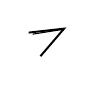
\begin{tikzpicture}\draw[line width=.7pt] (0,.3)--(.45,.35)--(.15,0);\draw (.05,.28)--(.43,.34);\end{tikzpicture}}
\mspage{22}
\figure{\begin{tikzpicture}\draw (0,0)..controls(.05,.22)and(.22,.18)..(.4,.19);\end{tikzpicture}}
\scanpage{24}
Soit $\mathcal E$ la catégorie des ensembles finis, avec comme
morphismes les applications \uline{injectives}. On
considère des foncteurs
\[
\mathcal E\xrightarrow{F}(\mathrm{Ens})
\]
tels que $\forall E\in\operatorname{Ob}\mathcal E$, $\operatorname{card}(F(E))$ est fini, i.e. des
foncteurs
\[
\mathcal E\longrightarrow(\mathrm{Ens}_f)
\]
Ils forment une catégorie $\uline{\operatorname{Hom}}(\mathcal E,(\mathrm{Ens}_f))$,
qui est un para-topos. Parmi ses objets, on
en distingue deux sortes particulières

a) Les foncteurs \uline{représentables} $\mathcal E\mathbin{\text{---}}(\mathrm{Ens})$.
de la forme
\[
h_I:E\longmapsto\operatorname{Hom}_{\mathcal E}(I,E)=\operatorname{Mon}(I,E)
\]
où $I$ est un ensemble fini. Le foncteur
\[
I\longrightarrow h_I\qquad\mathcal E^o\longrightarrow\uline{\operatorname{Hom}}(\mathcal E,(\mathrm{Ens}_f))
\]
est pleinement fidèle, et identifie $\mathcal E^o$ à
une sous-catégorie pleine de $\uline{\operatorname{Hom}}(\mathcal E,(\mathrm{Ens}_f))$

b) Les foncteurs de la forme
\[
H_I:E\longrightarrow\operatorname{Hom}_{(\mathrm{Ens})}(I,E)=E^I=H(I,E)
\]
(restrictions à $\mathcal E\subset(\mathrm{Ens}_f)$ des foncteurs
correspondants sur $(\mathrm{Ens}_f)$).

\uline{Prop} Les $h_I\in\operatorname{Ob}\overbrace{\uline{\operatorname{Hom}}(\mathcal E,(\mathrm{Ens}_f))}^{\mathcal H}$ sont des
objets connexes (non vides) de $\mathcal H$. À isomorphisme
\mspage{23}
\scanpage{25}
près, ce sont les composantes connexes des
foncteurs de la forme $H_J$.

\uline{Foncteurs spéciaux} $\mathcal E\mathbin{\text{---}}(\mathrm{Ens}_f)$ : ce sont les
foncteurs qui sont \inserted{isom. à des} sommes disjointes finies
de foncteurs de la forme $h_I$ --- ou encore
qui sont des \unsure{sommandes|sommants} directs
(pour $I$ de cardinal assez grand) des
foncteurs de la forme $H_I$.

\uline{Stabilités} Toute somme finie, \inserted{et} produit
fini \inserted{(plus gén. les $\varprojlim$ finies)} de foncteurs spéciaux est spécial.
Tout foncteur spécial $\mathcal E\mathbin{\text{---}}(\mathrm{Ens}_f)$ prend
ses valeurs dans la sous-catégorie
$\mathcal E$ de $(\mathrm{Ens}_f)$, i.e. \deleted{\unsure{donne}}\inserted{définit un} $\in\uline{\operatorname{Hom}}(\mathcal E,\mathcal E)$
(et on identifie par abus de langage
le foncteur $\mathcal E\longrightarrow(\mathrm{Ens}_f)$ avec $\mathcal E\mathbin{\text{---}}\mathcal E$)
Avec cette convention, le composé de
deux foncteurs spéciaux est spécial.
\mspage{24}
\scanpage{26}
\uline{Foncteurs distingués} : \inserted{Sommes disjointes finies de} quotient d'un foncteur
\deleted{\unsure{spécial par.}} $h_I$ par un groupe d'autom, i.e.
foncteurs isomorphes à des \inserted{sommes finies de} foncteurs de la
forme
\[
E\longmapsto\operatorname{Mon}(I,E)/H
\]
où $H\subset\mathfrak S_I$. Ce sont aussi les sommes
finies de composantes connexes de foncteurs
de la forme $H(I,E)/H=\operatorname{Hom}_{\mathrm{Ens}}(I,E)/H$.
Ces foncteurs ont les \unsure{$=^{s}$|mêmes} propriétés de
permanence que celles vues pour les
foncteurs spéciaux.

\margin{Tout foncteur \uline{distingué} est
isom. à un foncteur
de la forme
\[
E\longmapsto\coprod_{n\geq0}\operatorname{Mon}(I_n,E)\mathbin{\wedge}_{\mathfrak S_n}X_n
\]
où $\forall n$, $X_n$ est un $\mathfrak S_n$-ens. fini (\unsure{à g.}).}

Un hom \inserted{$u:F\longrightarrow G$} de foncteurs $F,G:\mathcal E\longrightarrow(\mathrm{Ens})$
est dit une équivalence s'il satisfait la
condition suivante

($\unsure{\sigma|\alpha}$) $\exists n\in\mathbf N$ tel que pour \deleted{deux} tout
ensemble fini $E$ \deleted{$\unsure{F}$} de cardinal $\geq n$, \deleted{et les \unsure{appl.}}
\deleted{\unsure{inj.} $E\hookrightarrow F$ \unsure{on a} $\unsure{F(E)\simeq G(E)}$,}
on a $u(E):F(E)\simeq G(E)$. On a

a) Si $F\mathrel{\overset{u}{\text{---}}}G\mathrel{\overset{v}{\text{---}}}H$ et si deux parmi les
trois $u,v,vu$ sont des équivalences, aussi le $3^\circ$.

b) Les \deleted{\unsure{morphismes}} équivalences sont stables par
chgt de base
\mspage{25}
\scanpage{27}
\[
\mathord{\text{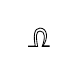
\begin{tikzpicture}[x=1ex,y=1ex,baseline=0,line width=.3pt]
\draw(0,0)--(.60,0)..controls(.45,.8)and(.48,1.5)..(1.0,1.5)..controls(1.65,1.5)and(1.70,.6)..(1.25,.02)--(1.8,.02);
\draw(0,-.05)--(.80,-.05)..controls(.65,.8)and(.65,1.25)..(1.0,1.25)..controls(1.45,1.25)and(1.45,.65)..(1.18,-.05)--(1.8,-.05);
\end{tikzpicture}}}=\uline{\operatorname{End}}(\mathcal E,\mathcal E)\subset\uline{\operatorname{Hom}}(\mathcal E,\mathrm{Ens})=\widehat{\mathcal E^o}
\]
$\mathord{\text{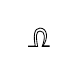
\begin{tikzpicture}[x=1ex,y=1ex,baseline=0,line width=.3pt]
\draw(0,0)--(.60,0)..controls(.45,.8)and(.48,1.5)..(1.0,1.5)..controls(1.65,1.5)and(1.70,.6)..(1.25,.02)--(1.8,.02);
\draw(0,-.05)--(.80,-.05)..controls(.65,.8)and(.65,1.25)..(1.0,1.25)..controls(1.45,1.25)and(1.45,.65)..(1.18,-.05)--(1.8,-.05);
\end{tikzpicture}}}$ est la sous-catégorie (pas pleine!) de $\widehat{\mathcal E^o}$ \unsure{formée}

a) comme objets,
des foncteurs $F:\mathcal E\mathbin{\text{---}}(\mathrm{Ens})$ qui se factorisent
par la sous-catégorie $\mathcal E$ de $\mathrm{Ens}$, i.e. tels que

$1^\circ$) $F(E)$ est fini pour tt $E\in\operatorname{Ob}\mathcal E$

$2^\circ$) $F(u)$ est injectif $\forall(u:E\mathbin{\text{---}}F)\in\operatorname{Fl}(\mathcal E)$

b) comme morphismes $F\xrightarrow{u}G$, des seuls
hom fonctoriels tels que $u(E):F(E)\mathbin{\text{---}}G(E)$ soit
injectif pour tt $E\in\operatorname{Ob}\mathcal E$.

$\mathord{\text{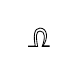
\begin{tikzpicture}[x=1ex,y=1ex,baseline=0,line width=.3pt]
\draw(0,0)--(.60,0)..controls(.45,.8)and(.48,1.5)..(1.0,1.5)..controls(1.65,1.5)and(1.70,.6)..(1.25,.02)--(1.8,.02);
\draw(0,-.05)--(.80,-.05)..controls(.65,.8)and(.65,1.25)..(1.0,1.25)..controls(1.45,1.25)and(1.45,.65)..(1.18,-.05)--(1.8,-.05);
\end{tikzpicture}}}$ a des opérations $\amalg,\times,\circ$
\[
\left\{\begin{aligned}
(F\unsure{+|\amalg}G)(E)&=F(E)\amalg G(E)\\
(F\times G)(E)&=F(E)\times G(E)\\
(F\circ G)(E)&=F(G(E))
\end{aligned}\right.
\]
\mspage{26}
\scanpage{28}
Sur Topos loc. annelé (commutativement) $X$, on a
\[
K(X,*)=\unsure{\sum|\bigoplus}_{n\geq0}K(B_{\mathfrak S_{nX}})
\]
On a pour $\xi\in K(X)$
\[
\tau^*(\xi)=\sum\tau^n(\xi)\in1+K(X,*)^{\wedge+}=1+\xi+\tau^2\xi\ \text{---}
\]
Pour $\xi\unsure{=|\in}\operatorname{cl}_{K(X)}(E)$, on a
\[
\tau^n(\xi)=\operatorname{cl}_{K(B_{\mathfrak S_{nX}})}\overset{n}{\bigotimes}E
\]
Ceci posé, on a la relation
\[
\tau^n(\xi)=\sum_{\substack{(\alpha_1,\ldots,\alpha_n)\in\mathbf N^n\\1\alpha_1+2\alpha_2+\cdots+n\alpha_n=n}}
\Sigma_{\alpha_1,\ldots,\alpha_n}(\lambda^1\xi,\ldots,\lambda^n\xi)\rho_1^{\alpha_1}\cdots\rho_n^{\alpha_n}
\]
\margin{Si $\xi$ est effectif,
s'agit-il d'un
\unsure{sommant} \unsure{direct}?
(Relation avec le
th. de commutation
\unsure{à la|de la} H. Weyl --- $\unsure{\xi}$?)}

$\rho_i\in K(B_{\mathfrak S_i})=R_{\mathbf Z}(\mathfrak S_i)$ est l'élément
unité de $K(B_{\mathfrak S_i})$, regardé comme él. de
degré $i$ dans
\[
R(1,\unsure{*})=K(e,*)=\sum_{i\geq0}R(\mathfrak S_i)
\]
\diagram{\begin{tikzcd}[ampersand replacement=\&,row sep=small]e\arrow[d]\\\text{topos ponctuel}\end{tikzcd}}
(de sorte que $\rho_1^{\alpha_1}\cdots\rho_n^{\alpha_n}$ est un élément de
$R(1,n)=R(\mathfrak S_n)$), et $\deleted{\unsure{\Sigma_{\alpha_1,\ldots,\alpha_n}}}$
\[
\Sigma_{\alpha_1,\ldots,\alpha_n}\in\mathbf Z[S_1,\text{---},S_n]
\]
est le polynôme \inserted{isobare de poids $n$ ($S_i$ étant de poids $i$)} qui exprime la fonction
symétrique à $n$ variables
\[
\begin{aligned}
&\sum(x_1\text{---}x_{\alpha_1})(x_{\alpha_1+1}\text{---}x_{\alpha_1+\alpha_2})^2\text{---}
\bigl(x_{\unsure{\alpha_1+\cdots+\alpha_{n-1}+1}}\cdots\unsure{x_{\alpha_1+\cdots+\alpha_n}}\unsure{)}^{\unsure{n}}\\
&=\sum x_1^{\unsure{\nu_1}}\text{---}x_n^{\unsure{\nu_n}}\quad(\text{où }\alpha_i=\text{nb des }\nu_j\text{ égaux à }i)
\end{aligned}
\]
comme polynôme en les fonctions sym.
élémentaires $S_1,S_2,\ldots,S_n$ en
\mspage{27}
\scanpage{29}
\uline{Corollaire} \deleted{On a $\lambda$} $\lambda^n(\xi)$ apparaît comme
coefficient de $\rho_1^n$ dans $\tau^n$; $S^n(\xi)$ (opération
de Adams) comme coefficient de $\rho_n$.
\figure{\begin{tikzpicture}\draw (0,0)--(0,-1.6);\end{tikzpicture}}

[\uline{NB} Il est facile \unsure{sans doute} de vérifier que
les $1_{K(X)}.\rho_1^{\alpha_1}\text{---}\rho_n^{\alpha_n}$ sont lin. indép. sur $K(X)$
dans $K(X,*)$ \ldots]

\uline{Question} Pour quels anneaux $k$ est-il
vrai que $R_k(1,*)=\sum R_k(\mathfrak S_n)$ est
l'anneau de polynômes \inserted{sur $\mathbf Z$} \unsure{engendré} par
les $\rho_i$ $(i\geq1)$? Est-ce vrai
si $k$ est un anneau local (plus
gén, tel que $K(k)\xleftarrow{\sim}\mathbf Z$)?
\mspage{28}
\scanpage{30}
jeu de go complet (sur go-ban $\unsure{v|\nu}\times\unsure{v|\nu}$)

noir joue $N$ coups

blanc joue $N'$ coups
\[
N=N'\text{ ou }N'+1
\]
\[
\boxed{N=P+Q}\qquad\boxed{N'=P'+Q'}\qquad\text{i.e. }\boxed{\varepsilon\overset{\mathrm{def}}{=}N-N'=\underset{\margin{\text{si blanc joue dernier}}}{0}\text{ ou }1}\ \deleted{\unsure{et}}
\]
\diagram{$\begin{array}{ll}
P&\text{nb de pièces noires sur go-ban en fin de partie}\\
P'&\text{---}\quad\text{blanc}\quad\text{---}\\
Q&\text{nb de prisonniers noirs}\\
Q'&\text{nb de prisonniers blancs}\\
T&\text{territoire noir}\\
T'&\text{territoire blanc}
\end{array}$}
\[
\boxed{P+P'+T+T'=\unsure{v|\nu}^2}
\]
\[
\begin{array}{ll}
\text{pts de noir}&Q'+T=\deleted{\unsure{N}}S\\
\text{pts de blanc}&Q+T'=\deleted{\unsure{N'}}S'
\end{array}
\]
Différence
\[
\begin{aligned}
\underbrace{D}_{=S-S'}&=(Q'+T)-(Q+T')=(Q'-Q)+(T-T')\\
&=(P-P')+(T-T')\unsure{-|+}\varepsilon
\end{aligned}
\]
\[
D+\unsure{v|\nu}^2=2(P+T)\unsure{-|+}\varepsilon
\qquad\text{ou}\qquad \unsure{v|\nu}^2-D=2(P'+T')+\varepsilon
\]
\[
(D'\overset{\mathrm{def}}{=}-D=S'-S)
\]
\[
\boxed{D=2(P+T)-\unsure{v|\nu}^2\unsure{-|+}\varepsilon}
\]
\[
(D'=2(P'+T')-\unsure{v|\nu}^2+\varepsilon)
\]
\mspage{29}
\scanpage{31}
Supposons qu'il y a des territoires
constitués de blanc et noir, considérés
\unsure{indélogeables}, blanc a joué dernier
(alors c'est à noir de jouer) on a
joué $n$ coups
\[
n=p+q\qquad\deleted{\unsure{n}}n'=p'+q'\qquad n=n'
\]
\margin{$p$ : nb de pions noirs sur goban
qui ne sont prisonniers virtuels}

$q$ nb de prisonniers virtuels

$t$ territoire noir (\unsure{avec pris enlevé} les pris. bl.)

$t'$ \ldots\ blanc (\text{---} noirs)
\margin{$p+p'+t+t'=\unsure{v|\nu}^2$}
\[
\begin{array}{ll}
\deleted{\unsure{Q}}\ s=t+q'&\text{pts de noir potentiels}\\
s'=t'+q&\text{---}\quad\text{blanc}\quad\text{---}
\end{array}
\]
\[
d=s-s'=(t-t'\unsure{,}+(q'-q)=(t-t')+(p-p')
\]
\[
\unsure{v|\nu}^2+d=2(p+t)\qquad\text{i.e.}\qquad\boxed{d=2(p+t)-\unsure{v|\nu}^2}
\]
\[
D=d\unsure{-|+}\varepsilon\qquad\varepsilon=0,1\qquad(\mathrm{NB}\quad p+t=P+T)
\]
\margin{?}
\figure{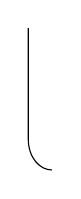
\begin{tikzpicture}\draw (0,1.8)--(0,.4)..controls (0,.15) and (.15,0)..(.3,0);\end{tikzpicture}}
Comme on ne peut prévoir la valeur de
$\varepsilon$ (est-elle indépendante de la suite du
jeu?) il est raisonnable de compenser
l'avantage de noir (de commencer)
en posant $\varepsilon=1$ (i.e. en admettant que
noir joue dernier)
\mspage{30}
\scanpage{32}
Un pion ne peut se placer en position de ``prise'', i.e.
sur une intersection libre telle qu'il n'ait plus
\inserted{aucune} \deleted{de} liberté (i.e. que le groupe qui le contient
n'ait plus de liberté) sauf dans les deux
cas suivants:

1°) Cas du ``Ko'' cf plus bas

2°) Cas de ``remplissage d'un trou'' : \deleted{disons que}
$A$ joue, sur une \deleted{\unsure{case}} \inserted{intersection $i$} qui est la seule liberté restante
d'un ensemble \inserted{$E$ réunion} de groupes de $B$ \inserted{(groupement de $B$)}, de façon que
toutes les libertés du groupe $G$ de $A$ contenant $i$
soient prises par des pions de $E$. ($E$ est entouré
par les pions de $A$ sauf en $i$, et $E$ entoure
le groupe \inserted{$G$} de $A$ contenant $i$)

\deleted{\unsure{Commençant à}}

\deleted{Chaque} \inserted{Les} joueurs prennent \deleted{\unsure{à tour de}} \inserted{à tour de} rôle, et ils ne
peuvent sauter leur tour (obligation de jouer).
L'obligation de jouer tombe dans le seul cas
suivant:

(fin de partie) Le joueur $A$ n'a plus de case
libre où il soit légitime de se mettre (\inserted{i.e.} où il
\unsure{n'en|n'y} soit pas en état de prise, sans \deleted{l'}\inserted{une des} exceptions
1° et 2° plus haut), sauf des \deleted{cases} \inserted{intersections $c$} du type
suivant: il y a un groupement $E$ de $A$
n'ayant plus que deux libertés \deleted{\unsure{intérieures}} \inserted{en $\unsure{i_1,i_2}$}
\deleted{\unsure{ces deux libertés}}
\mspage{31}
\scanpage{33}
\deleted{entourées de pions de $A$}
(toutes les autres libertés étant prises par des
pions de $B$) \inserted{et celles-ci étant intérieures (\unsure{i.e.} entourées de pions de $A$)} et $c$ est une de ces deux-là.

[\uline{NB} si $A$ s'y mettait, dès au prochain coup
$B$ en \uuline{se} plaçant dans la \deleted{\unsure{autre}} dernière liberté
$c'$ disponible du groupement $E'=E\cup\{c\}$, capturerait
$E'$ --- et de proche en proche il capturerait
tous les pions de $A$ !\deleted{\unsure{]}} , \unsure{$=$|même} si $A$ avait
un avantage considérable sur $B$ par les
territoires couverts !] On exige de plus,
cependant, que le groupement $E$ soit
``indélogeable'', i.e. que si c'était le
tour de $B$ de jouer au lieu de $A$, il ne
pourrait se poser ni en $c$, ni en $c'$
(i.e. que l'on ne peut trouver un sous-
groupement $E_c$ de $E$ \inserted{entourant $c$} dont $c$ soit la
seule liberté \deleted{\unsure{inté}} restante, (\deleted{pas de} \inserted{ou, ce qui revient \unsure{au $=$|au même}} le groupe-
ment $E_{c'}$ de $E$ entourant $c'$ dont $c'$ soit
la seule liberté restante), ni que $B$
puisse poser en $c$ ou $c'$ par la règle du
Ko.
\mspage{32}
\scanpage{34}
En fin de partie

noir a $\rho$ groupements solidaires \inserted{$G_i$} (avec chacun
$\unsure{\gamma_i|y_i}\geq2$ yeux

blanc : $\rho'$ groupements solidaires \inserted{$G'_j$} ($\ldots$ $\unsure{\gamma'_j|y'_j}\geq2$)

\deleted{Si blanc joue dernier ($\varepsilon=0$) alors les $\rho'$
groupements ont chacun exactement 2
yeux, donc $\unsure{T'|t'}=2\rho'$}

Si $t-2\rho\leq t'-2\rho'$
alors c'est blanc qui joue le dernier
(i.e. $\varepsilon=0$, i.e. $D=d$)

Si $t'-2\rho'<t-2\rho$,
c'est noir qui joue le dernier
(i.e. $\varepsilon=1$, i.e. $D=d-1$)
\mspage{33}
\scanpage{35}
\margin{Groupes formels}
\mspage{34}
\scanpage{36}
\uline{Groupes formels}

\textcircled{I} Extension d'un $p$-divisible par un lisse (\unsure{ou unipotent}) est triviale

\uline{Cor} Extension d'un $p$-divisible a-torique par un lisse (\unsure{ou unipotent})
est un \deleted{\unsure{extension}} \inserted{produit}

[Tout \unsure{sous-groupe} $p$-divisible a-torique est central

Tout groupe quotient \inserted{$p$-div.} a-torique est abélien avec un
plus grand sous-groupe $p$-divisible a-torique
--- qui est néc. central $\ldots$

\unsure{formuler} sort des \deleted{\unsure{plus}} grds sous-gps $p$-divisibles
a-toriques :
$\left\{\begin{array}{l}
\text{existe}\\
\text{stabilité par ext. corps de base}\\
\text{inclusion, sous sous-groupes}\\
\text{$p$-div$^{\mathrm{les}}$, sous groupes quotients}
\end{array}\right.$

\uline{NB} Pour qu'un grp. formel soit a-torique il faut,
\unsure{que la repr. lin. soit} \unsure{unipotente}.]

\uline{Rem} $(G_{\mathrm{ab}})/\operatorname{Im}\unsure{\delta|d}=\pi_0$ n'a pas de partie a-torique i.e. est \uline{linéaire}.

\margin{\unsure{résulte aussitôt du} \unsure{fait que} $\unsure{(G/R)_{\mathrm{ab}}|G/R}\unsure{\simeq|\to}G/R$ \unsure{est linéaire}. \uline{NB} \uline{\unsure{Mais}} \unsure{Centre} $(G/\operatorname{Cent}G)$ est quasi unipotent}

\textcircled{II} Extension d'un groupe formel [lisse] par un $p$-divisible est
\inserted{[si $G$ lisse]} \deleted{\unsure{triviale}} un produit --- à isogén. près du moins$\ldots$

\uline{Cor} $DG\cap Z(G)$ est \unsure{quasi-unipotent} i.e. annulé par une
puiss. de $p$. [Même, \deleted{$\unsure{G|Z(G)}$} $\operatorname{Cent}(\operatorname{D\acute{e}r}G)$ est quasi-unip.$^{\unsure{\times}}$]

[\uline{Dire} soit \deleted{\unsure{ainsi}} $T$ \inserted{la partie} $p$-divisible de \deleted{$\unsure{\operatorname{Cent}G|Z(G)}$} \inserted{$\operatorname{Cent}\operatorname{D\acute{e}r}G$}, \deleted{alors} \inserted{elle se \unsure{trouve} \unsure{dans $Z(G)$}}
\[
G\simeq\unsure{T'|T}\times G/T\inserted{\unsure{\phantom{T}'}}\quad
\text{donc}\quad DG\cap T=\{e\}
\]
]

\uline{Cor} $G$ (lisse) est \deleted{\unsure{produit}} \inserted{(isogénie)} de la pure partie a-torique par un \unsure{linéaire|fibré}$\ldots$?

\uline{Question} $DG\cap Z(G)$ est-il \unsure{un} unipotent, i.e.
un \unsure{contenu} par du $H_p$ (\unsure{dans la th. de cls}) ?

\uline{Structure}

\diagram{\begin{tikzcd}[ampersand replacement=\&,column sep=small,row sep=small]
 \& \& L_1\arrow[r,"d"]\&L_0\arrow[dr]\& \&\\
1\arrow[r]\&\pi_1\arrow[ur]\arrow[dr]\& \& \&\pi_0\arrow[r]\&1\\
 \& \&D_1\arrow[r,dash,"\delta"]\&D_0\arrow[ur]\arrow[d,"\theta"]\&\&\\
 \& \& \& {[\operatorname{Aut}D_1]}\&\&
\end{tikzcd}}

\[
p^\infty\pi_1=e\qquad \operatorname{at}(\pi_0)=\{e\}
\]
\[
\left\{\begin{array}{ll}
L_1=Z(G),&D_1=D(G),\\
L_0=G/Z(G),&D_0=G/D(G),\\
\pi_1=L_1\cap D_1,&\pi_0=G/L_1D_1
\end{array}\right.
\qquad
\left\{\begin{array}{l}
D_1^{D_0}=\pi_1\\
\unsure{D_{1\,D_0}|(D_1)_{D_0}}=\{e\}
\end{array}\right.
\]

\unsure{se reconstruit} à partir
\[
\pi_1,\quad \operatorname{Im}d\times\operatorname{Im}\delta,\quad \pi_0
\]
\[
D'=D_1\amalg_{\pi_1}L_1\qquad L'=L_0\times_{\pi_0}D_0
\]
\margin{\uline{NB} $\operatorname{Im}\delta\simeq\widehat H$\quad $H$ grp. alg. canonique mod. is. \unsure{étale}}

[obstruction nulle dans $H^3(\pi_0,\pi_1)$

indétermination dans $H^2(\pi_0,\pi_1)$]

Traiter cas $\pi_0$ $p$-divisible (plus gén., description des
\unsure{fibres} \unsure{groupes} de $G$ \unsure{images inverses} de $p^\infty\pi_0$

\uline{Dire quels sont les} $L_1\xrightarrow{d}L_0$ possibles
$(D_1\xrightarrow{\delta}D_0,\theta)$ ---
\margin{(\deleted{\unsure{détermination}} \inserted{Conditions sur $\pi_1,\pi_0$} \unsure{\ldots})
$\unsure{(\ker\delta)^{D_0}|(\ker\delta)}=\pi_1$,
$\unsure{(\ker\delta)_{D_0}}\simeq\{0\}$}

\margin{\unsure{NB}}
\uline{Condition pour que} $G$ soit linéaire
\inserted{\unsure{DG div. comm. et algébrisable}$\ldots$}
\mspage{35}
\scanpage{37}
Dans la situation générale des ext. pour $G$ correspondant
à une extension

\diagram{\begin{tikzcd}[ampersand replacement=\&,column sep=small]
1\arrow[r,dash]\&\pi_1\arrow[r,dash]\&G_1\arrow[r,dash,"d"]\&G_0\arrow[r,dash]\arrow[d,dashed,"\theta"]\&\pi_0\arrow[r,dash]\&1\\
\&\&\&\operatorname{Aut}(G_1,\pi_1)\&\&
\end{tikzcd}}

on a (pour le $G$ donné) un hom
\[
\operatorname{Cent}(G_0)\cap\operatorname{Ker}\theta\xrightarrow{\varphi_G}Z^1(\pi_0,\pi_1)
\]
dont le noyau est l'image de $Z(G)$ dans $G_0$.

\margin{$\overbrace{\underbrace{\pi_0,\operatorname{Im}d}_{G_0},\pi_1}^{G}$}

Dans le cas qui nous intéresse
\[
\begin{aligned}
\relax[\ G_1&=D'=L_1.D_1=\operatorname{Cent}G.\operatorname{Der}G,\quad
G_0=L'=G/L_1\cap D_1\\
&=G/\operatorname{Cent}G\cap\operatorname{Der}G\quad ---\ ]
\end{aligned}
\]
cela \deleted{\unsure{aussi}} s'exprime par
\[
\operatorname{Cent}(D_0)\cap\operatorname{Ker}\theta\xrightarrow{\varphi_G}\operatorname{Hom}(\pi_0,\pi_1)
\]
\inserted{(c'est ce qui exprime que $L_0\longleftrightarrow\operatorname{Cent}G$ est iso)}
dont le noyau doit être nul; ceci montre
donc qu'on doit avoir (compte tenu
que $\pi_1$ est quasi-unipot.)
\[
\boxed{\operatorname{Cent}D_0\cap\operatorname{Ker}\theta\text{ est quasi-unipotent}}
\]
\inserted{$\simeq[\operatorname{Cent}(\operatorname{D\acute{e}r}(G))/\operatorname{Cent}(G)]\cap\operatorname{Cent}D'_0$}
\margin{$D_0\simeq G/\unsure{(\operatorname{Cent}G)}$}

En fait, on doit avoir mieux, comme
\unsure{à savoir} \uline{$\operatorname{Cent}(D_0)$ unipotent}

\diagram{\begin{tikzcd}[ampersand replacement=\&,column sep=small,row sep=large]
\&\&L_1\arrow[dl,dash,hook',"A"']\arrow[dr,dash,hook',"H"]\arrow[drr,bend left=40,dash,"D_0"]\&\&\\
1\arrow[r,dash,hook]\&\pi_1=L_1\cap D_1\arrow[rr,dash,hook,"A\times H"]\arrow[dr,dash,hook,"H"']\&\&D'\arrow[r,dash,hook]\&G\\
\&\&D_1\arrow[ur,dash,hook,"A"']\arrow[urr,bend right=40,dash,"L_0"']\&\&
\end{tikzcd}}
\margin{\unsure{donc}}
\mspage{36}
\scanpage{38}
\[G/Z\]
\[p^\infty\operatorname{Cent}(G/Z)\]
\diagram{\begin{tikzcd}[ampersand replacement=\&]
\uline{\operatorname{Hom}}(\pi,Z)\\
G\arrow[u,"\unsure{\varphi}"]
\end{tikzcd}}
\[\deleted{\unsure{G}}\quad \underbrace{Z^{\unsure{1|\prime}}\times T}\]
\[\operatorname{Cent}(G/Z)\]
\[\deleted{\operatorname{Cent}(G/\unsure{\operatorname{Cent}})}\]
\[
\left\{\begin{array}{l}
\boxed{\operatorname{Cent}(\operatorname{Der}G)\quad\text{unipotent}}\\[5pt]
\deleted{\unsure{\text{liné}}}\quad\boxed{(G/Z)_{\mathrm{ab}}\quad\deleted{\text{\unsure{a-tori}}}\ \uline{\text{linéaire}}}\\[5pt]
\boxed{\operatorname{Cent}(G/Z)\quad\text{unipotent}}
\end{array}\right.
\]
\diagram{\begin{tikzcd}[ampersand replacement=\&]
|[draw,rounded corners=18pt,inner xsep=14pt,inner ysep=8pt]|{(\operatorname{D\acute{e}r}G)_{\mathrm{ab}}\quad\text{unipotent ?}}\arrow[r]\&\text{\unsure{voire|quasi} fini}
\end{tikzcd}}
\[\deleted{\operatorname{Der}G_{\mathrm{ab}}\unsure{\neq|=}\unsure{\operatorname{Div}}}\]
\mspage{37}
\scanpage{39}
\mspage{38}
\margin{$\unsure{G|g}$\quad $\unsure{Z}$\quad $\unsure{G}$}

\diagram{\begin{tikzcd}[ampersand replacement=\&,column sep=small,row sep=small]
\&Z\arrow[dr,dash]\&\&\&\\
\unsure{\mathfrak z}=Z\cap DG\arrow[ur,dash]\arrow[dr,dash,"H"']\&\&Z.DG\arrow[r,dash]\&G\arrow[r,dash]\&\unsure{\mathcal G|G}\\
\&DG\arrow[ur,dash]\&\&\&
\end{tikzcd}}
\[\underbrace{Z.DG\;---\;G}\]
\[---\;\underbrace{Z\cap DG\;---\;DG\;---\;Z.DG}\;---\;G\]
\[DG\qquad G/Z\]
\[DG/Z\cap DG\qquad 1\]

\diagram{\begin{tikzcd}[ampersand replacement=\&]
1\arrow[r,dash]\&\mathfrak z\arrow[r,dash]\&\mathbb D\arrow[r,dash]\&\widehat{\mathbb H}\arrow[r]\&1
\end{tikzcd}}

$H$ groupe alg. linéaire connexe (lisse)

$D^{\unsure{3|\mathfrak z}}$ \inserted{groupe formel divisible (lisse)}
extension centrale de $\widehat H$ par $\mathfrak z$

\deleted{\unsure{groupe formel}\quad\unsure{commutatif}}
\inserted{$\mathfrak z$ groupe formel \unsure{com.}}

$\mathfrak z\longrightarrow Z$ hom. de groupes formels
commutatifs
\scanpage{40}
\diagram{\begin{tikzcd}[ampersand replacement=\&,row sep=small,column sep=small]
H\&H_T\arrow[l]\&H_T^i\& W\supset W_i\\
\widehat G\arrow[d]\&\widehat G_T\arrow[l]\arrow[d]\&\&\\
I\&T\arrow[l]\&W\&\\
\&T_i\&\&
\end{tikzcd}}
\figure{\begin{tikzpicture}\draw[->] (4,1.6)--(4,0)--(0,0);\end{tikzpicture}}

\diagram{\begin{tikzcd}[ampersand replacement=\&]
1\arrow[r,dash]\&H\arrow[r,dash]\&E\arrow[r,dash]\&G\arrow[r,dash]\&1
\end{tikzcd}}
\[\varphi(x,y)\]
\[
\varphi(x,y)\deleted{\unsure{\varphi}}\,(\unsure{\varphi(y,x)|\varphi(x,y)})^{-1}=\unsure{\varphi_{x,y}|\varphi xy}
\]
\[\Psi(x+y)-\Psi(x)-\Psi(y)=\varphi(x,y)\]

\diagram{\begin{tikzcd}[ampersand replacement=\&]
1\arrow[r]\&\widehat G_a\arrow[r,dash]\arrow[d,dash,"\unsure{\simeq}"]\&E\arrow[r]\&\widehat G_a\arrow[r,dash]\&1\\
\&Z(E)=D(E)\&\&\&
\end{tikzcd}}
\[\unsure{H_a}\]

\diagram{\begin{tikzcd}[ampersand replacement=\&]
\deleted{\unsure{\widehat G}}\arrow[r,dash]\&\unsure{G'}\\
\unsure{\mathfrak z} \&
\end{tikzcd}}

\[
\begin{array}{cc}
[Z\longrightarrow A]&[Z\longrightarrow A]\\
\unsure{\simeq} &\unsure{\simeq}\\
\relax[D\longrightarrow L]&\widehat{[D\longrightarrow L]}
\end{array}
\]

\diagram{\begin{tikzcd}[ampersand replacement=\&,column sep=small,row sep=small]
\&Z\arrow[r]\&A\arrow[dr,"\unsure{?}"]\&\\
\unsure{\pi_0|\pi_1}\arrow[ur,"\unsure{?}"]\arrow[dr,"\unsure{\sim}"']\&\&\&\pi_0\\
\&D\arrow[r]\&L\arrow[ur,"?"']\&
\end{tikzcd}}
\[ [\downarrow] \]
\diagram{\begin{tikzcd}[ampersand replacement=\&,column sep=small,row sep=small]
\&Z\arrow[r,dash]\&A\arrow[dr,dash]\&\\
\pi_1\arrow[ur,dash]\arrow[dr,dash]\&\&\&\pi_0\\
\&\widehat D\arrow[r,dash]\&\widehat L\arrow[ur,dash]\&
\end{tikzcd}}

\diagram{\begin{tikzcd}[ampersand replacement=\&,row sep=small]
Z\arrow[r]\&A\\
\widehat D\arrow[r]\arrow[u,phantom,"\unsure{\simeq}"]\&\widehat L\arrow[u,phantom,"\unsure{\simeq}"]\\
Z\arrow[r,dash]\&A\\
D\arrow[r,"0"']\&L
\end{tikzcd}}

\[\deleted{\unsure{\Phi}(x,y)=}\]
\[
\uline{\Phi}(x,y)=\underbrace{\varphi(x,y)}_{\unsure{\varphi}}+
\underbrace{\Psi(x+y)-\Psi(x)-\Psi(y)}
\]
\[H^2(G_a,G_a)\]
\mspage{39}
\scanpage{42}
$G$ groupe alg. lisse connexe sur $k$, ayant une décomposition en ext. de Chevalley
(p.ex. $k$ parfait)
\[
1\longrightarrow\deleted{\unsure{H}}\inserted{L}\longrightarrow G\longrightarrow A^{\unsure{\mathrm{ab}}}\;---\;1
\qquad (*)\quad A\text{ schéma abélien},\ L\text{ groupe alg. affine lisse connexe}
\]
Considérons de plus $M=G_{\mathrm{aff}}$, le plus grand quotient affine de $G$,
et la suite
\[1\;---\;Z\;---\;G\longrightarrow\deleted{\unsure{A}}M\longrightarrow1\]
on sait que $(**)$ $M$ affine, $Z_{\mathrm{aff}}=1$ (\unsure{caractéristiques} pour cette ext.
et que cela entraîne $Z$ central dans $G$, $Z\longrightarrow A$ \uline{épi}.

Considérons
\diagram{\begin{tikzcd}[ampersand replacement=\&,column sep=small,row sep=small]
\&\&1\arrow[dr]\&\&\&\&1\\
\&\&\&L\arrow[dr,hook]\arrow[rr,dashed]\&\&M\arrow[ur]\\
(\mathrm D)\&L\cap Z=\mathfrak z\arrow[urr,hook]\arrow[drr,hook]\&\&\&G\arrow[ur]\arrow[dr]\&\\
\&\&\&Z\arrow[ur,hook]\arrow[rr]\&\&A\arrow[dr]\\
\&\&1\arrow[ur]\&\&\&\&1
\end{tikzcd}}

avec $Z\longrightarrow A$ épi, donc $G=Z.L$, i.e. $L\;---\;M$ épi.

$G$ est une extension centrale de $A\times M$ par $\mathfrak z$, et est connu (comme
telle, avec reconstitution du diagramme (D)) par la connaissance
des deux extensions centrales $L$ de $M$ par $\mathfrak z$ et $Z$ de $A$ par $\mathfrak z$.
Donc la donnée de $G$ \deleted{\unsure{(avec sa décomposition}} \inserted{(satisfaisant l'hyp. du} début équi-
vaut à celle de

a) des groupes alg. $M,A,\mathfrak z$ ($M$ affine lisse connexe, $A$ V.A., $\mathfrak z$ \inserted{affine} commutatif)

b) d'extensions \uline{centrales} $L$ de $M$ par $\mathfrak z$, et $Z$ de $A$ par $\mathfrak z$, satisfaisant

(i) $L$ lisse connexe,\quad (ii) $Z_{\mathrm{aff}}=1$

On peut reformuler ces données en

a') groupe alg. affine lisse connexe $L^{\unsure{*}}$, et V.A. $A$

b') ss-groupe \inserted{alg.} $\mathfrak z\subset\operatorname{Cent}(L)$

c') Extension \deleted{\unsure{de}} \inserted{centrale} $Z$ de $A$ par $\mathfrak z$ telle que $Z_{\mathrm{aff}}=1$.

On sait déterminer les ext. centrales d'un schéma abélien $A$
par un groupe \inserted{alg.} comm. affine $\mathfrak z$ par
\[
\operatorname{Ext}^1(A,\mathfrak z)=\operatorname{Hom}(D(\mathfrak z),\uline{\operatorname{Pic}}_{A/k})
\]
(la catégorie de ces extensions est rigide puisque le
$\operatorname{Ext}^0=\operatorname{Hom}(A,\mathfrak z)=0$) donc la donnée \deleted{de} \inserted{d'une extension} $Z$ équivaut à
la donnée de
\[\varphi:D(\mathfrak z)\longrightarrow\uline{\operatorname{Pic}}_{A/k}\]
et il reste à expliciter la condition $Z_{\mathrm{aff}}=1$, \deleted{\unsure{par suite}} \inserted{(plus gén.}
\mspage{41}
\scanpage{43}
à déterminer $Z_{\mathrm{aff}}$ en termes de $\varphi$, et écrire ensuite qu'il est 1).
On voit \deleted{que} aisément que $Z_{\mathrm{aff}}$ est un quotient \inserted{$\mathfrak z_1$} de \deleted{\unsure{$\varphi$}} $\mathfrak z$
--- savoir le plus grand quotient de $\mathfrak z$ tel que l'extension
correspondante de $A$ par $\mathfrak z_1$ \deleted{\unsure{y}} soit triviale, et c'est aussi,
$\mathfrak z_1=D(\operatorname{Ker}\varphi)$, donc il faut exprimer $\operatorname{Ker}\varphi=1$.

\deleted{\unsure{On}} Il y a deux cas à distinguer, en décomposant
$\mathfrak z=\underbrace{\mathfrak z_u}_{\mathrm{unipot.}}\times\underbrace{\mathfrak z_m}_{\mathrm{t.\ mult.}}$,
et posant $\Gamma=D(\mathfrak z_m)$

1°) $k$ de car. 0, donc $\mathfrak z_u$ est un groupe vectoriel, \deleted{Alors} $\varphi$
\inserted{soit $\mathfrak z_u=W(t)$ ($t$ tangent à l'origine)}
correspond à deux hom
\[
\varphi_0:\deleted{\unsure{\mathfrak z_u\longrightarrow}}\ t\longrightarrow
 t_{\uline{\operatorname{Pic}}_{A/k}}\simeq H^1(A,\uline O_A)
\]
\[
\varphi_{\deleted{\unsure{m}}1}:\uline\Gamma\longrightarrow\uline{\operatorname{Pic}}_{A/k}
\]
\deleted{Si $t_0=\operatorname{Ker}\unsure{\varphi}$}

Il faut $\varphi_0$ injectif, $\varphi_1$ injectif. (donc la donnée de
$\mathfrak z=\mathfrak z_u\times\mathfrak z_m$ \inserted{et de l'extension $Z$ telle que $Z_{\mathrm{aff}}=1$} équivaut, par dualité, à la donnée d'un \inserted{couple}
\deleted{\unsure{sous espace}} $(\unsure{\Lambda|A},\Gamma)$ d'un \deleted{\unsure{un}} sous-espace vect. de $H^1(A,\uline O_A)=$
$t_{\uline{\operatorname{Pic}}_{A/k}}$ et d'un sous-groupe constant dans \deleted{(de t.f.}
\deleted{\unsure{de pt de tors}} à engendrement fini de $\uline{\operatorname{Pic}}_{A/k}$)

2°) $k$ de car. pos. Alors \deleted{\unsure{si}} il est bien connu que
$(Z_{\mathrm{aff}})_u$ \deleted{est} est isogène à $\mathfrak z_u$, ce qui montre que si
$(Z_{\mathrm{aff}})_u=0$, $\mathfrak z_u$ est fini; \unsure{(et on|et on} est plus à l'aise pour
manipuler $D(\mathfrak z_u)$, \deleted{\unsure{Donc on doit avoir}}
\inserted{les groupes alg. comm. finis unipotents}
correspondant par dualité exactement aux groupes alg. comm. \uline{radiciels}.
\deleted{$\varphi_0:D(\mathfrak z_u)$}

Ici la donnée de $\varphi$ équivaut à
\[
\varphi_0:D(\mathfrak z_u)\longrightarrow\uline{\operatorname{Pic}}_{A/k}
\qquad\text{(se factorise par $\uline{\operatorname{Pic}}^0=A^*$}
\]
\[\text{et même par $\widehat{A^*}$)}\]
\[
\varphi_1:\uline\Gamma\longrightarrow\uline{\operatorname{Pic}}_{A/k}
\]
et la condition $Z_{\mathrm{aff}}=1$ équivaut à : $\varphi_0$, $\varphi_1$ injectifs.

(Donc la donnée de $\mathfrak z=\mathfrak z_u\times\mathfrak z_m$, $\mathfrak z_u$ fini, et de l'ext. $Z$ équivaut
à la donnée d'un couple $(\tau,\uline\Gamma)$, d'un sous-groupe alg.
radiciel $\tau$ de $\uline{\operatorname{Pic}}_{A/k}$ et d'un sous-groupe constant libre
$\uline\Gamma$ de $\uline{\operatorname{Pic}}_{A/k}$, pour avoir $D(\mathfrak z)=\tau\times\uline\Gamma\hookrightarrow\uline{\operatorname{Pic}}_{A/k}$
\mspage{42}
\scanpage{44}
\uline{NB} Les groupes $\mathfrak z$ qui peuvent intervenir (pour $G$ connexes
satisfaisant la condition de Chevalley) sont \deleted{\unsure{ceux}} les groupes
alg. comm. affines pour lesquels a) $\exists$ mono \inserted{central} $\mathfrak z\hookrightarrow L$,
avec $L$ lisse connexe affine --- tjrs vérifié, et \unsure{$=$|même} avec
$L$ commutatif --- ce qui donnera un $G$ commutatif ---
et b) $\exists$ schéma abélien $A$ et mono $D(\mathfrak z)\hookrightarrow\uline{\operatorname{Pic}}_{A/k}$, ce
\deleted{\unsure{qui est nécessaire}} \inserted{qui} (pour $k$ alg. clos, pour simplifier)

1°) si $\operatorname{Car}k=0$, \deleted{\unsure{par}} est \uline{tjrs} vérifié

2°) si Car. $k=p>0$ est vérifié sss $\mathfrak z_u$ fini.

\margin{\unsure{cette} note \unsure{élémentaire|est triviale} sur ce point}

\uline{NB} Ceci \deleted{montre} \inserted{\unsure{pour inégales caractéristiques}} \deleted{que} la construction de $G_{\mathrm{aff}}$ \deleted{n'est pas \unsure{cat}} (pour $G$
groupe affine lisse à fibres connexes sur base $S\ldots$) n'est pas
de nature ``constructible en général''. Prenons p.ex. pour $G$
une extension d'un schéma abélien $A$ par $G_a$, non triviale
en un pt maximal \deleted{\unsure{y}} de $S$ de car. 0, donc $(G_\unsure{y|\eta})_{\mathrm{aff}}=1$, cependant
aux \deleted{\unsure{pts}} spécialisations $s$ de $y$ de car. $p>0$, on aura $(G_s)_{\mathrm{aff}}\simeq G_a$.
Par contre, cela montre en \unsure{$=$|même} temps qu'en égalis. car.
résiduelles, c'est une construction \inserted{de nature} ``constructible''.

\uline{Reformulation} Il est maladroit de prendre $\mathfrak z\subset\operatorname{Cent}(L)$ et
\uline{mono} \deleted{\unsure{a}} $D(\mathfrak z)\hookrightarrow\uline{\operatorname{Pic}}_{A/k}$, il vaut mieux dire qu'on se
donne

A) groupe alg. affine lisse connexe $L$ et V.A. $A$

B) extension de $A$ par $\operatorname{Cent}(L)$ i.e. hom.
\[D(\operatorname{Cent}(L))\longrightarrow\uline{\operatorname{Pic}}_{A/k}\]

L'avantage de la présentation adoptée plus haut semble
uniquement dans le fait qu'elle permet d'expliciter
la donnée B) sans faire intervenir des ``schémas'' à la
Cartier trop dégueulasses ---
\mspage{43}
\scanpage{45}
\margin{Fourbis auxiliaires\\
cohomologiques\\
pour groupes\\
Formels}
\mspage{44}
\scanpage{46}
\mspage{1}

I \quad $(N,M,d,\theta)=C$

\deleted{$\unsure{\theta:M\longrightarrow\operatorname{Aut}_{\mathrm{gr}}(N)}$}

\deleted{$\unsure{\beta:C'\longrightarrow C}$}

II \quad $(N',M',d',\theta')=C'_{\unsure{1}}$

III \quad $\text{\textcircled{$\beta$}}\left\{
\begin{array}{l}\pi_0(C)\simeq\pi_0(C'_{\unsure{1}})\\
\pi_1(C)\simeq\pi_1(C'_{\unsure{1}})
\end{array}\right.$ compatibles aux op. de $\pi_0$ sur $\pi_1$

\diagram{\begin{tikzcd}[ampersand replacement=\&,column sep=small,row sep=small]
\&N\cap N'=z=\pi_1\arrow[dl,dash]\arrow[dr,dash]\&\\
N\arrow[dr,dash]\arrow[ddr,dash,bend right=50,"M'"']\&\&N'\arrow[dl,dash]\arrow[ddl,dash,bend left=50,"M"]\\
\&NN'=H\arrow[d,dash]\&\\
\&G\&
\end{tikzcd}}

problème de reconstitution pour $K=G/z\simeq\operatorname{Im}(G\to M\times M')$
et $H=\operatorname{Im}(N\times N'\to G)$

\diagram{\begin{tikzcd}[ampersand replacement=\&,column sep=small]
\& (N\times N'\underset{\unsure{z}}{\longrightarrow}G,D_1,\Theta_1)\arrow[dl]\arrow[dr]\&\\
(N,M,d,\theta)\arrow[dr]\&\&(N',M',d',\theta')\arrow[dl]\\
\&(G,M\times M',D_2,\Theta_2)\&
\end{tikzcd}}
\[
(H,K,D,\Theta)
\]

\diagram{\begin{tikzcd}[ampersand replacement=\&,column sep=small]
1\arrow[r,leftrightarrow]\&z\arrow[r]\&H\arrow[r,dash,hook]\&G
\end{tikzcd}}
\figure{\begin{tikzpicture}[x=.8cm,y=.35cm]
\draw (1,1)--(1,1.5)--(3,1.5)--(3,1);\draw(0,0)--(0,-.5)--(2,-.5)--(2,0);
\end{tikzpicture}}

\diagram{\begin{tikzcd}[ampersand replacement=\&,column sep=large,row sep=large]
H\arrow[rrr,bend left=20]\&N\times N'\arrow[l]\arrow[r]\&M\times M'\arrow[d]\&K\arrow[l]\arrow[d]\\
\pi_1\arrow[u]\&\pi_1\times\pi_1\arrow[u]\arrow[l,"\text{épi}"']\&\pi_0\times\pi_0\arrow[r]\&\pi_0
\end{tikzcd}}
\quad cocart \qquad cart
\[
(\alpha,\alpha').(\lambda,\lambda')=(\alpha.\lambda,\alpha'.\lambda')
\]
\[
(\alpha,\alpha').(\lambda,-\lambda)=(\alpha.\lambda,-\alpha'\lambda)
\]

Obstruction dans $H^3(B_{\pi_0}/X,\pi_1)$

Indétermination dans $\begin{array}{c}H^2(B_{\pi_0}/X,\pi_1)\\ \Vert\\ \operatorname{Ext}_{\mathrm{gr}}(\pi_0,\pi_1)\end{array}$

\hrulefill

\deleted{\unsure{A}}
\[
\left\{\begin{array}{l}
N'\text{ central}\ \inserted{\text{i.e. }N'\subset\operatorname{Cent}(G)}
\Longleftrightarrow\uline{\theta':M'\longrightarrow\operatorname{Aut}_{\mathrm{gr}}(N')\text{ triviale}}\quad(\text{d'où }N'\text{ commut})\\
N\text{ cocentral}\ \inserted{\text{i.e. }N\supset DG}\Longleftrightarrow M'\text{ commutatif}
\end{array}\right.
\]

L'ensemble des deux conditions signifie que
la donnée de $C'$ se réduit à la donnée
de groupes comm. $N'$ et $M'$ et un
hom
\[
N'\xrightarrow{d'}M'
\]
sans plus. Cela implique que l'opération
de $\pi'_0$ sur $\pi'_1$ est triviale, donc itou pour
$\pi_0$ sur $\pi_1$ (condition à mettre sur $C$)
ceci dit, la donnée de
\[
\boxed{\begin{array}{cc}N'\xrightarrow{d'}M'&d'(x')\text{ \uline{central}}\\&N'\text{ commutatif}\end{array}}
\]
pour \textcircled{A} est sans condition
de compatibilité supplémentaire

\margin{\deleted{Lieber \unsure{Edgar},\par
Wie die lieben Leute sich miteinander vergnügen --- ob allein, zu zwein, zu drei, zu \unsure{vier|fünf} oder zu zwanzig}}
\margin{$\deleted{\unsure{H(\beta)}}$}
\mspage{45}
\scanpage{47}
\mspage{2}

Condition pour que $N'=\uline{\operatorname{Cent}}G$

\unsure{a|*}) Il faut que $N'\subset\uline{\operatorname{Cent}}G$, i.e. op. \inserted{$\theta'$} de $M'$ sur $N'$
triviale ($\Longrightarrow N'$ commutatif et $d'(N')\subset\uline{\operatorname{Cent}}(M')$)

b) D'ailleurs, l'image du centre de $G$ dans $K$ \inserted{$=G/\pi_1$} est
contenue dans $\uline{\operatorname{Cent}}(K)$ \inserted{$\supset N'/\pi_1$ i.e. son image dans $M$ contenue dans $\uline{\operatorname{Cent}}(K)/(N'/\pi_1)$}, et aussi dans
$\operatorname{Ker}(\theta:M\longrightarrow\uline{\operatorname{Aut}}_{\mathrm{gr}}(N))$. Soit
\[
\zeta=\deleted{\uline{\operatorname{Cent}}(M)}\inserted{\uline{\operatorname{Cent}}(K)/(N'/\pi_1)}\cap\operatorname{Ker}\theta
\]
et soit $\overline{N}'$ \deleted{\unsure{son}} l'image inverse dans $G$ \inserted{le ss-groupe invariant de $G$ \unsure{déf.}},
\inserted{$(N'\subset\uline{\operatorname{Cent}}(G)\subset\overline{N}')$}
qui est donc
une extension de $\zeta$ par $N'$. L'opération de
$G$ sur $\overline{N}'$, via $M$, par automorphismes, est triviale
sur $\unsure{N'}$ et sur $\zeta=\overline{N}'/N'$ \inserted{(car $\zeta\subset\uline{\operatorname{Cent}}(M)$)}, donc se définit par un
hom
\[
M\longrightarrow\uline{\operatorname{Hom}}_{\mathrm{gr}}(\zeta,N')
\]
prenant en fait ses valeurs dans $\uline{\operatorname{Hom}}_{\mathrm{gr}}(\zeta,\pi_1)$
\deleted{$\unsure{\operatorname{Hom}_{\mathrm{gr}}(M,\pi_1)}$}
(lequel, par construction de $\zeta$, est aussi trivial
sur $d(N)\subset M$ ($\zeta\subset\operatorname{Ker}\theta$). Donc l'hom
se factorise en
\[
\varphi_G:\pi_0\longrightarrow\uline{\operatorname{Hom}}_{\mathrm{gr}}(\zeta,\pi_1)
\qquad\deleted{\unsure{Z^1}}
\]
qui s'interprète \inserted{aussi} comme
\[
\psi_G:\zeta\longrightarrow\uline{\operatorname{Hom}}_{\mathrm{gr}}(\pi_0,\pi_1)
\qquad\deleted{\unsure{\operatorname{Hom}_{\mathrm{gr}}}}
\]
Soit $\zeta_G=\operatorname{Ker}\psi_G$, et $\overline{N}'_G$ l'image inverse de
$\zeta_G$ dans $G$, il est clair alors que
\[
\overline{N}'_G=\uline{\operatorname{Cent}}(G)
\]
donc $N'=\uline{\operatorname{Cent}}(G)$ équivaut à la condition
\[
\boxed{\zeta_G=\operatorname{Ker}\psi_G=1\quad\text{i.e. }\psi_G\text{ injectif}}
\]

Soit $G_1$ une deuxième sol. du Pb initial,
différant de $G$ par une extension \deleted{$\unsure{E}$} $E$ de $\pi_0$ par $\pi_1$
(op. triviale de $\pi_0$ sur $\pi_1$ i.e. extension centrale),

\margin{\uline{\unsure{donc plus}} :
\diagram{\begin{tikzcd}[ampersand replacement=\&,column sep=small,row sep=small]
\zeta=\operatorname{Ker}\theta\cap\operatorname{Cent}M\arrow[d]\\
Z^1(\pi_0,\pi_1)
\end{tikzcd}}
$M\simeq G/N'$\par
$\zeta\subset\unsure{\zeta'}=\operatorname{Im}\uline{\operatorname{Cent}}(K)$}
\mspage{46}
\scanpage{48}

U N I V E R S I T E\par
DES SCIENCES ET TECHNIQUES\par
\uline{DU LANGUEDOC}\par
AMC/MD

Montpellier, le 19 juin 1975

\uline{Diffusion} : Liste A\par
n° 3979

AVIS DE SOUTENANCE D'UNE THESE DE DOCTORAT DE\par
\uline{SPECIALITE BIOLOGIE ANIMALE}

\uline{Nom et prénom du candidat} : MARTEAU Marie

\uline{Titre de la thèse} : Systématique et biologie des acanthocéphales du genre
CORYNOSOMA LUHE 1904.

\uline{Date, heure et lieu de soutenance prévus} : Jeudi 26 juin à 10 heures, salle de
cours n° 5 - U.S.T.L.

\uline{Nom des Directeurs de thèse} : M. EUZET - M. GOLVAN

\uline{Désignation du laboratoire où la thèse est préparée} : Laboratoire de parasitologie
comparée U.S.T.L. et laboratoire de parasitologie C.H.U. St Antoine PARIS.

\uline{Analyse de l'ouvrage} : L'étude anatomique des Acanthocéphales du genre \uline{Corynosoma}
permet de reprendre la systématique des espèces décrites. On démontre que l'on
peut séparer les espèces parantes de cetacés et celles qui vivent dans les
oiseaux marins. On reprend le cycle biologique des Corynosoma et on discute
le phénomène de capture par les poissons. On émet une hypothèse sur la phyllogenèse
des espèces étudiées.

\uline{Durée approximative des recherches ayant abouti à la thèse} : 2 ans

\uline{Composition du jury proposé} :\quad\begin{tabular}[t]{l}M. EUZET\\M. BOUIX\\M. CHABAUD\\M. GOLVAN\end{tabular}

Le Secrétaire Général,

\unsure{E. Siau}
\figure{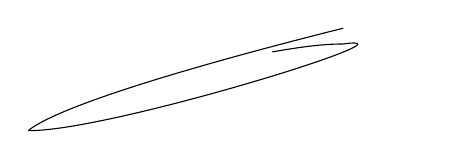
\begin{tikzpicture}[x=1cm,y=1cm]
\draw (0,0) .. controls(.5,.4) and(3,1.05)..(4,1.3);
\draw (0,0).. controls(1,-.02)and(5.1,1.25)..(4.0,1.1)..controls(3.7,1.1)and(3.4,1.05)..(3.1,1.0);
\end{tikzpicture}}
\uline{E. SIAU}

\begin{tabular}{ll}
MR\quad LE PROFESSEUR GROTHENDIECK A.&\\[1em]
MATHEMATIQUES&5-856
\end{tabular}

\mspage{47}
\scanpage{49}
\mspage{3}
\diagram{\begin{tikzcd}[ampersand replacement=\&]
1\arrow[r,dash]\&\pi_1\arrow[r,dash]\&E\arrow[r,dash]\&\pi_0\arrow[r,dash]\&1
\end{tikzcd}}

Les autom intérieurs de $E$ sont l'identité sur
$\pi_0$ et $\pi_1$, donc définissent des hom $\pi_0-\pi_1$,
et on trouve ainsi un accouplement
\[
c_E=c_{G,G_1}:\quad\pi_0\times\pi_0\longrightarrow\pi_1
\]
(associant à $x,y\in\pi_0$ : $\bar{x}\bar{y}\bar{x}^{-1}\bar{y}^{-1}$ \inserted{$\in\pi_1$}; où $\bar{x},\bar{y}$ relèvent
$x$ et $y$) C'est une forme alternée, nulle ssi
l'extension $E$ est commutative. On doit
trouver, au \uline{signe} près
\[
\psi_{G_1}=\psi_G+\deleted{\unsure{\beta}}\widetilde c_E\alpha.
\]
où $\widetilde c_E:\pi_0\longrightarrow\uline{\operatorname{Hom}}(\pi_0,\pi_1)$ est défini de façon
évidente par $c_E$ (choix de la droite ou la \uline{gauche}
correspondant au \deleted{\unsure{choix}}\inserted{changement} d'un \uline{signe} !), $\alpha$
l'hom de passage au quotient
\diagram{\begin{tikzcd}[ampersand replacement=\&]
\zeta\arrow[r,dash]\arrow[rr,bend right=30,"\alpha"']\&M\arrow[r,dash]\&\pi_0
\end{tikzcd}}

\deleted{$\beta:\uline{\operatorname{Hom}}(\pi_0,\pi_1)\longrightarrow\uline{\operatorname{Hom}}(\pi_0,N')$
déduit de l'inclusion $\pi_1\hookrightarrow N'$.}
Il faut donc
se borner aux $G_1$ i.e. aux $E$ pour lesquels
$c_E$ est tel que
\[
\psi_G+\deleted{\unsure{\beta}}\widetilde c_E\alpha:\zeta\longrightarrow\uline{\operatorname{Hom}}(\pi_0,\pi_1)
\]
soit injectif.

\deleted{On peut simplifier encore cette condition,
en notant \deleted{\unsure{ici}} que la composée
\diagram{\begin{tikzcd}[ampersand replacement=\&,column sep=small]
\zeta\arrow[r,"\psi_{G_1}"]\&\uline{\operatorname{Hom}}(\pi_0,N')\arrow[r,dash]\&\uline{\operatorname{Hom}}(\pi_0,N'/\pi_1)
\end{tikzcd}}
ne dépend pas du choix de $G_1$ : c'est}

\margin{\uline{NB} on suppose $\pi_0$ commutatif ?!\par
\unsure{Que faire} sinon ? Regarder l'image $\pi_0^*$ de $\zeta$ dans $\pi_0$, invariant et central\par
on trouve $\pi_0^*\times\pi_0\longrightarrow\pi_1$}
\mspage{48}
\scanpage{50}

U N I V E R S I T E\par
DES SCIENCES ET TECHNIQUES\par
DU LANGUEDOC\par
------------\par
AMC/GJ

Montpellier, le 5 Juin 1975

\uline{Diffusion} : Liste A\par
N° 3510

\uline{AVIS DE SOUTENANCE D'UNE THESE DE DOCTORAT DE}\par
\uline{SPECIALITE : MATHEMATIQUES APPLIQUEES}

\uline{Nom et prénom du candidat} : NANARD Marc

\uline{Titre de la thèse} : L'influence de l'agencement des E.S. sur les performances
d'un système d'exploitation.

\uline{Date, heure et lieu de soutenance prévus} : 16 Juin 1975 à 10 heures\par
Salle de Cours n° 9, U.S.T.L.

\uline{Nom du Directeur de thèse} : J. FALGUEIRETTES

\uline{Désignation du laboratoire où la thèse est préparée} :\par
Centre de Recherche en Informatique et Gestion.

\uline{Analyse de l'ouvrage} : On étudie l'influence de l'organisation des entrées
sorties sur le comportement du système. On examine en particulier le problème
du fonctionnement parallèle de l'U.C. et des canaux et le problème des conflits
d'accès disque. Les modèles proposés sont appliqués à un exemple concret.

\uline{Durée approximative des recherches ayant abouti à la thèse} : 2 ans 1/2

\uline{Composition du jury proposé} :\par
\begin{tabular}{l}J. FALGUEIRETTES\\Y. ESCOUFIER\\J.P. VERJUS\\C. KAISER\end{tabular}

LE SECRETAIRE GENERAL,

\unsure{E. Siau}
\figure{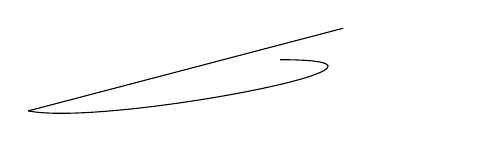
\begin{tikzpicture}[x=1cm,y=1cm]
\draw(0,0)--(4,1.05);\draw(0,0)..controls(1,-.2)and(5.4,.65)..(3.2,.65);
\end{tikzpicture}}
\uline{E. SIAU}

\begin{tabular}{ll}
MR\quad LE PROFESSEUR GROTHENDIECK A.&\\[1em]
MATHEMATIQUES&5-856
\end{tabular}

\mspage{49}
\scanpage{51}
\deleted{clair sur la formule précédente donnant $\psi_{G_1}$ en
termes de $\widetilde c_E$, mais on peut définir cet hom
\[
\psi_0:\zeta\longrightarrow\operatorname{Hom}(\pi_0,N'/\pi_1)
\]
en termes des données de départ (I II \uline{III})
qui définissent en fait un groupe $K\simeq G/\pi_1$
ext. \inserted{centrale} de $M$ par $N'/\pi_1$, d'où comme précédemment
\[
M\longrightarrow\uline{\operatorname{Hom}}(\zeta,N'/\pi_1)
\]
se factorisant par $\pi_0$, i.e.
\[
\zeta\xrightarrow{\psi_0}\uline{\operatorname{Hom}}(\pi_0,N'/\pi_1).
\]
Soit $\zeta_0=\operatorname{Ker}\psi_0$}

\mspage{4}

\margin{\deleted{\diagram{\begin{tikzcd}[ampersand replacement=\&,row sep=small]
\zeta\arrow[r,dash]\arrow[d,phantom,"\supset" description]\&\deleted{\unsure{\pi_0}}\uline{\operatorname{Hom}}(\pi_0,\pi_1)\\
\zeta_0\arrow[ur]\&
\end{tikzcd}}
$\pi_0^*=\zeta/\zeta_0\subset\pi_0$\par
$\pi_0^*\longleftrightarrow\uline{\operatorname{Hom}}(\pi_0,\pi_1)/\unsure{\zeta_0}$\quad\textcircled{inj}}}

\diagram{\begin{tikzcd}[ampersand replacement=\&]
\unsure{K}\arrow[r]\&\Sigma\\
I\arrow[u]\&
\end{tikzcd}}

On peut dévisser un peu plus en introduisant
\[
\zeta_0=\operatorname{Ker}(\zeta\longrightarrow\pi_0)
\]
\margin{$\begin{aligned}
&=\deleted{\unsure{\operatorname{Im}}}\ d(\operatorname{Cent}(N)\cap d^{-1}(\operatorname{Cent}M))\\
&=d(\operatorname{Cent}(N))\cap\operatorname{Cent}(M)\\
&\simeq\operatorname{Cent}(N)/\pi_1\cap\unsure{\operatorname{Cent}M}
\end{aligned}$}
et l'hom induit par $\psi_G$:
\[
\psi_{0\unsure{G}}:\zeta_0\longrightarrow\uline{\operatorname{Hom}}(\pi_0,\pi_1).
\]
\margin{?}
On trouve que la définition de celui-ci
ne dépend pas du choix de $G_1$, mais
\deleted{peut se faire en termes du groupe $H$
et $N,N'\subset H$ (construits par les données
I II III) Une condition préliminaire indépendante
de $G_1$ (i.e. de $E$) est que \textcircled{b} \uline{$\psi_0$ soit
injective}} --- cela exprime que $N'$ est \uline{égal}
au centre de $H$, $N'=\uline{\operatorname{Cent}}(H)$. Ceci
étant supposé acquis, \deleted{\unsure{pour}}\inserted{soit}
\margin{(annulé!)}
\mspage{50}
\scanpage{52}
\mspage{\unsure{5}}
\[
\overline\psi_{G_1}:\zeta/\zeta_0=\pi_0^*\longrightarrow\uline{\operatorname{Hom}}(\pi_0,\pi_1)/\zeta_0
\]
déduit de $\psi_{G_1}$ par passage au quotient.
La condition à exprimer encore est

c) $\overline\psi_{G_1}$ est injective

Cette condition dépend effectivement de
$G_1$ à priori, puisque $\psi_{G_1}$ donc $\overline\psi_{G_1}$ en
dépend (de la manière explicitée plus
haut). Cette condition sur $G_1$ i.e. sur
\[
E_{\unsure{G}}\in\operatorname{Ob}\ \uline{\operatorname{Ext}}_{\mathrm{gr}}(\pi_0,\pi_1)
\]
\margin{(annulé\unsure{?})}

\figure{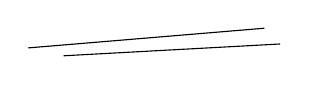
\begin{tikzpicture}\draw(0,0)--(3,.25);\draw(.45,-.1)--(3.2,.05);\end{tikzpicture}}

On veut exprimer maintenant
$N=DG$. Donc

 a) $N\supset DG$ i.e. $M'\ (=G/N)$ commutatif
\[
(\Longrightarrow\pi_0\text{ comm})
\]
Il faut exprimer ensuite que pour tout
ss-grpe \inserted{inv} $N_1\subset N$ tel que $G/N_1$ comm, on a
$N_1=N$. $G/N_1$ comm signifie que $G$ y
opère trivialt, cela implique qu'il opère
trivialt sur $N/N_1$ \inserted{et que celui-ci est comm}, or $G$ opère sur $N$
(ou $N/N_1$) via $M$, donc la condition est que
\deleted{$\unsure{N_1}$} $N/N_1$ est majoré par $\eta=N_{\unsure{\mathrm{comm}\,M|\mathrm{coinv}\,M}}$ \inserted{$=N/N_0$, i.e. $N_1\supset N_0$}.
Ceci dit dans l'extension \inserted{$G/N_0$} de $G/N=M'$ par
$\eta$, $G$ y opère, \inserted{en induisant l'id. sur les facteurs}, d'où un hom
\[
G\longrightarrow\uline{\operatorname{Hom}}(M',\eta)
\]
d'ailleurs nul sur $N$, d'où hom
\[
M'\longrightarrow\uline{\operatorname{Hom}}(M',\eta)
\]
\mspage{51}
\scanpage{53}
\mspage{6}
ou encore
\[
M'\times M'\xrightarrow{\lambda_G}\eta
\]
C'est obtenu ainsi : si $x,y\in M'(\unsure{\ell})$, on relève en
$\bar{x},\bar{y}\in\unsure{G|N}$, on prend $(\bar{x},\bar{y})=\bar{x}\bar{y}\bar{x}^{-1}\bar{y}^{-1}$, qui est
dans $N$, on réduit mod $N_0$, et c'est $\lambda_G(x,y)$.
(\deleted{\unsure{Comme}}\inserted{Si} $N'$ est central (ce qu'on suppose))
cette description montre que si $\unsure{\bar{x}}\ \unsure{\text{ou}|,}\ \unsure{\bar{y}}$
$\in d'(N')\subset M'$, alors \deleted{$\unsure{q}$} $\lambda_G(x,y)=0$, donc $\lambda_G$
s'interprète comme un hom
\[
\pi_0\otimes\pi_0\xrightarrow{\lambda_G}\eta=(N_{\mathrm{comm}})_M
\]
Notons aussi que $\lambda_G$ est alternée. Ceci
posé, \deleted{la condition} on a évidemment
\[
N/DG\simeq\eta/\lambda_G(\pi_0\otimes\pi_0)
\]
donc la condition cherchée est que
$\lambda_G$ \uline{est surjective}. Pour apprécier
cette condition, il faut voir comment
$\lambda_G$ varie avec $G$, on trouve (si $G_1$ \unsure{est à partir de|est déduit de}
$G$ défini par l'extension $E$ de $\pi_0$ par $\pi_1$)
\[
\lambda_{G_1}=\lambda_G+\beta c_E
\]
où $c_E:\pi_0\otimes\pi_0\longrightarrow\pi_1$ est l'accouplement
associé à l'ext. centrale de $\pi_0$ \inserted{(comm)} par $\pi_1$,
et où
\[
\beta:\pi_1\longrightarrow\eta=(N_{\mathrm{comm}})_M
\]
est le passage au quotient. \deleted{$\unsure{N_0}$}

Nous pouvons dévisser la condition
$\lambda_G$ \uline{surjective}, en introduisant encore
\mspage{52}
\scanpage{54}
\mspage{7}
$\eta_0=\operatorname{Coker}(\pi_1\longrightarrow\eta)$, et l'hom
\[
\lambda_0:\pi_0\otimes\pi_0\longrightarrow\eta_0
\]
déduit de $\lambda_G$ par passage au quotient. C'est
indépendant du choix de $G$, on le voit que
c'est ce qu'on construit directement dans
le groupe $K=G/\pi_1$. Il faut donc

b) $\lambda_0$ surjectif (car signifie aussi
que $N/\pi_1$ dans $K\subset M\times M'$ est $=DK$,
ou encore que $dN=DM\ \unsure{\}}$ exactement)
\margin{Vérifier}

\deleted{\unsure{a}} Introduisons alors $\operatorname{Ker}\lambda_0=P\subset\pi_0\otimes\pi_0$,
(indépendant de $G$), donc $\lambda_G$ induit
\[
\overline\lambda_G:P\twoheadrightarrow\pi_1^{\deleted{\unsure{*}}}{}_{\inserted{*}}=\operatorname{Im}(\pi_1\longrightarrow\eta)\subset\eta
\]
et la condition effective dépendant du
choix de $G$ qui reste à exprimer
est

c) $P\xrightarrow{\overline\lambda_G}\pi_1^{\deleted{\unsure{*}}}{}_{\inserted{*}}$ est un épi.

Ici la dépendance de cette condition
par $G$ variable est explicitée grâce à
la formule donnant $\overline\lambda_{\unsure{G_1}}$ en fonction
de $\lambda_G$, qui s'écrit de façon évidente
\[
\overline\lambda_{G_1}=\overline\lambda_G+pc_Ei
\]
$i$ l'inclusion $P\subset\pi_0\otimes\pi_0$, $p$ la projection $\pi_1\longrightarrow\pi_{1*}$.
\mspage{53}
